\section{Phân tích và thiết kế hệ thống}
Chương này tập trung trình bày về các use-case, quy trình nghiệp vụ của những chức năng cơ bản và thiết kế tổng quan cho kiến trúc hệ thống. Đây là cơ sở quan trọng giúp định hình trực tiếp quá trình xây dựng và phát triển hệ thống cả về mặt kĩ thuật lẫn nghiệp vụ.

\subsection{Sơ đồ usecase}
\begin{figure}[H]
	\centering
	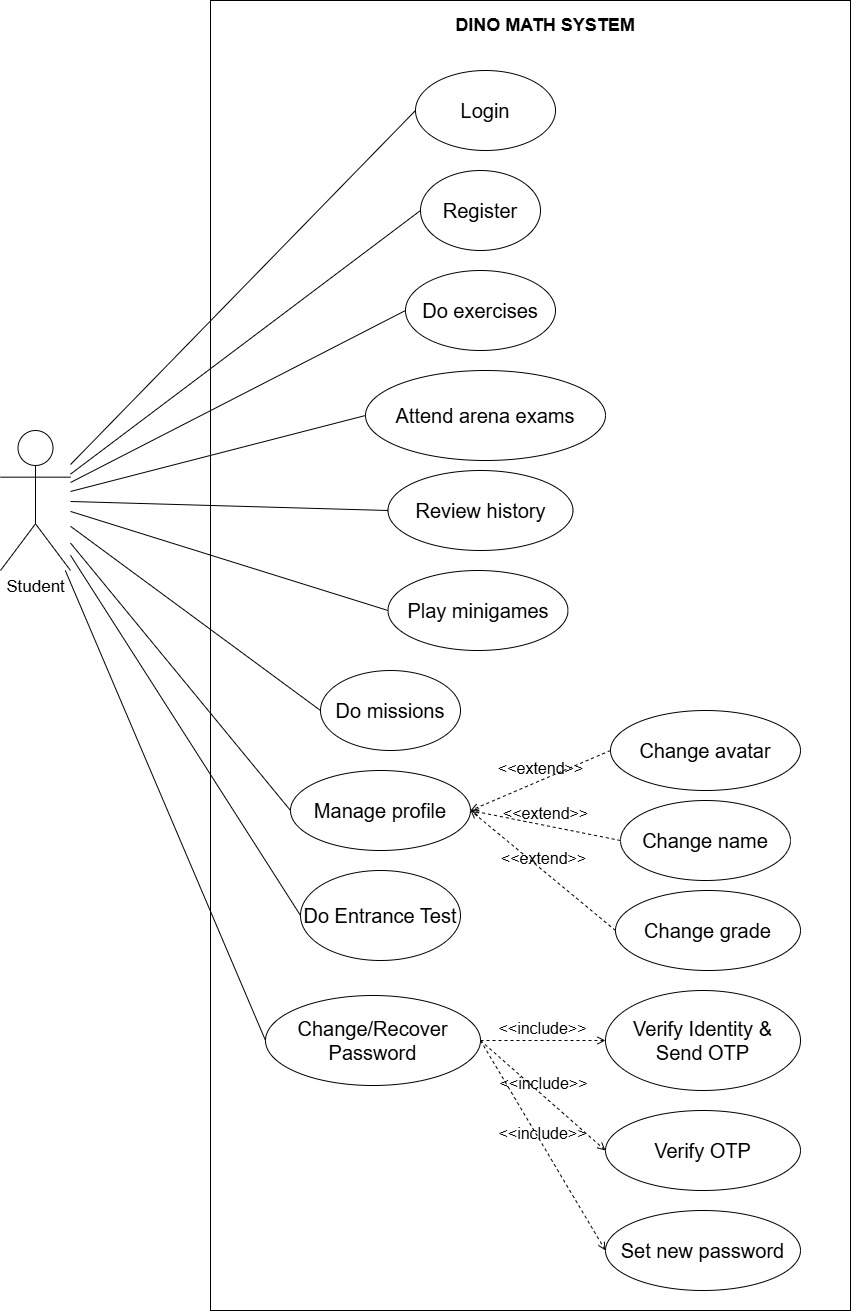
\includegraphics[width=0.8\textwidth]{Image/Diagrams/Usecase/StudentUseCase.jpg}
	\vspace{0.6cm}
	\caption{Usecase Diagram - Học sinh}
	\label{fig:studentuc}
\end{figure}
\begin{figure}[H]
	\centering
	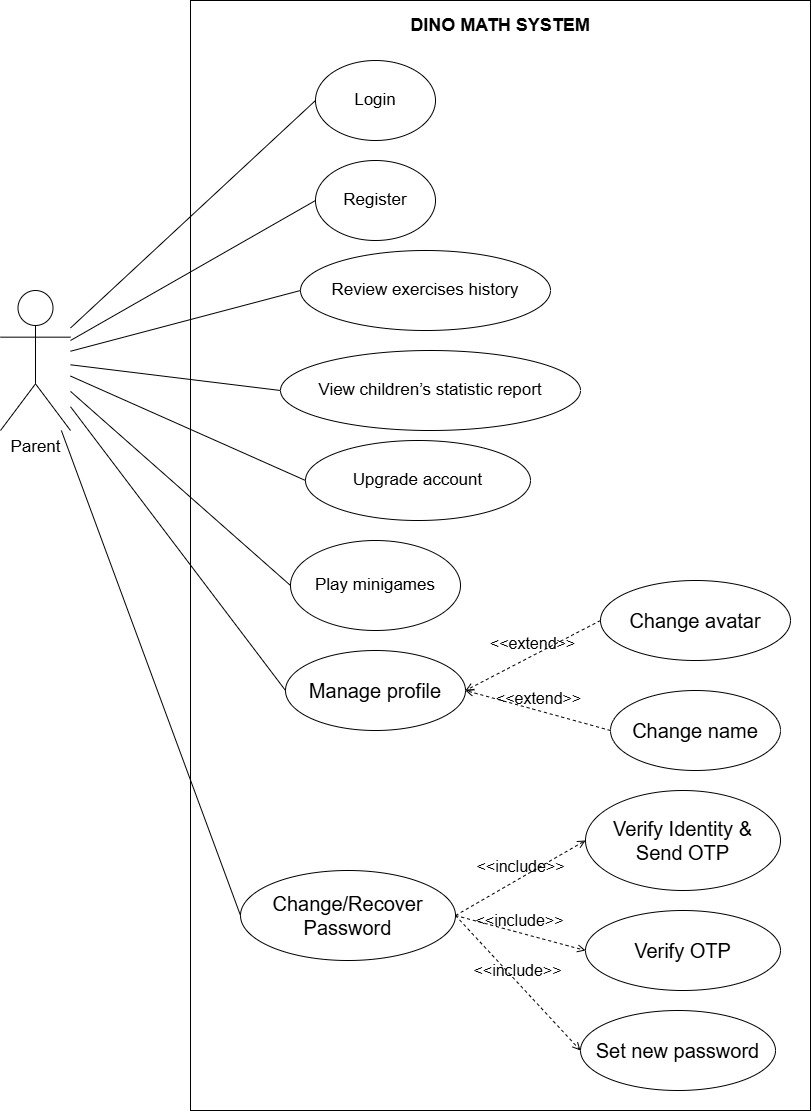
\includegraphics[width=0.8\textwidth]{Image/Diagrams/Usecase/ParentUseCase.jpg}
	\vspace{0.6cm}
	\caption{Usecase Diagram -  Phụ huynh}
	\label{fig:parentuc}
\end{figure}
\begin{figure}[H]
	\centering
	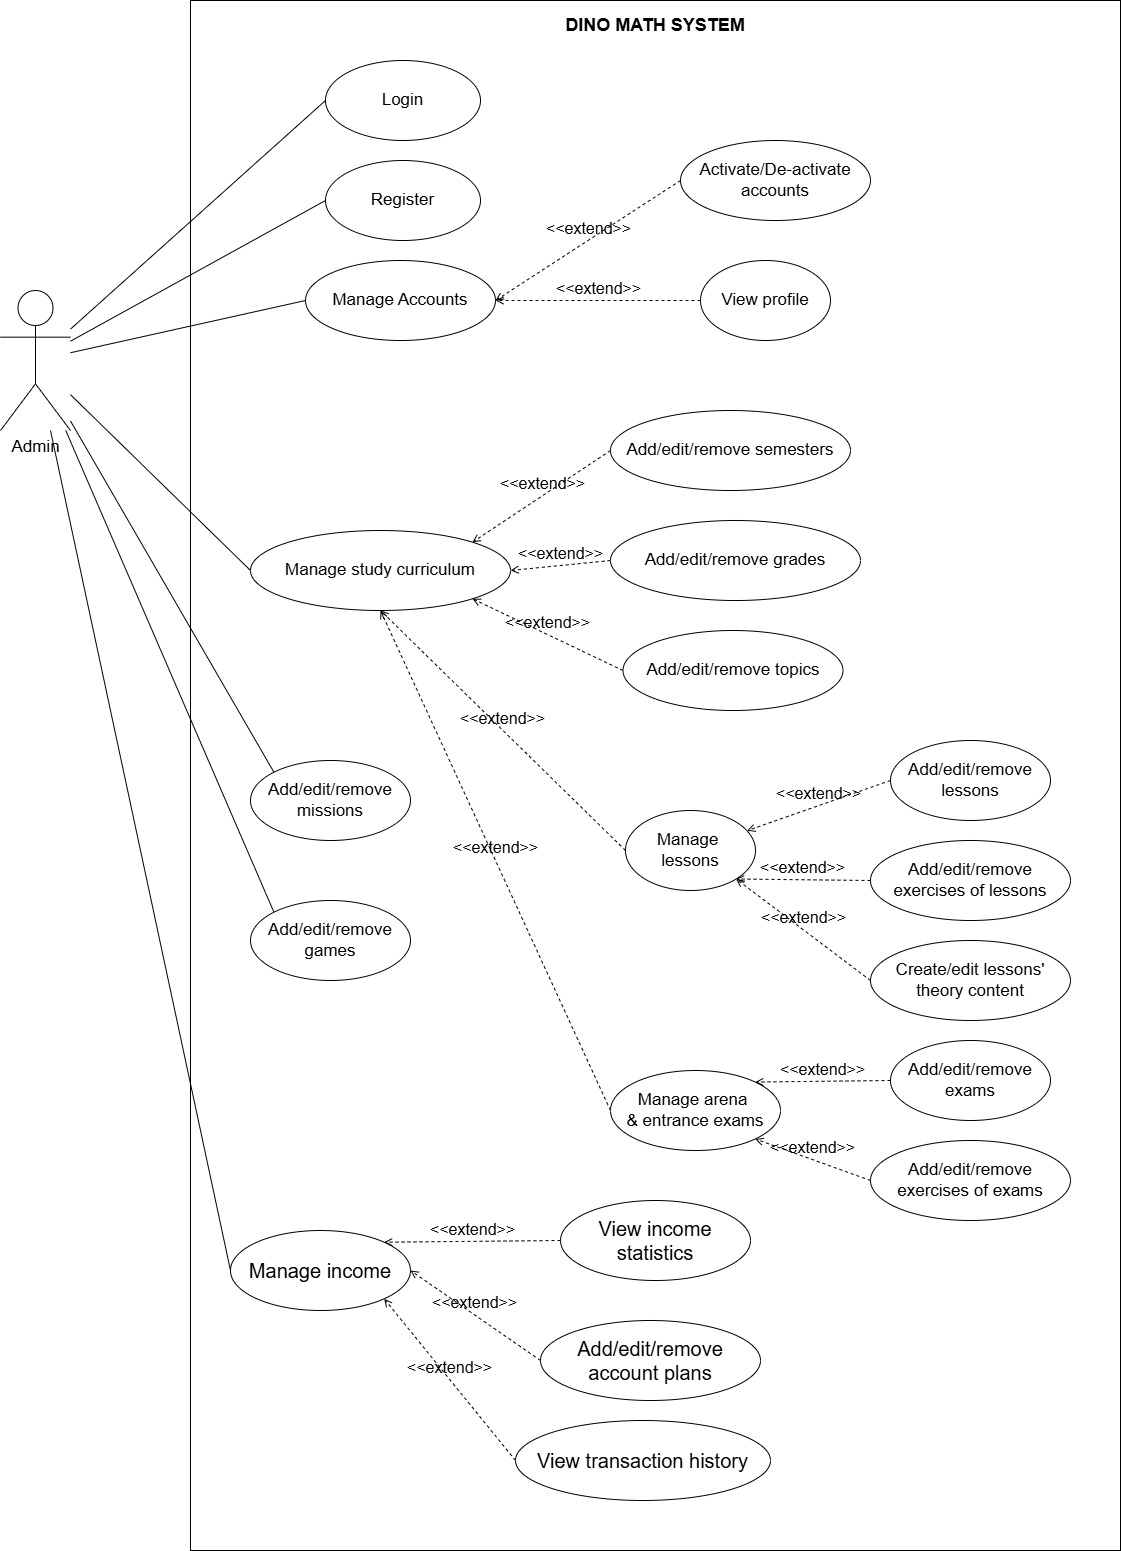
\includegraphics[width=0.9\textwidth]{Image/Diagrams/Usecase/AdminUsecase.jpg}
	\vspace{0.6cm}
	\caption{Usecase Diagram - Admin}
	\label{fig:adminuc}
\end{figure}

\subsection{Mô tả chi tiết}
\subsubsection{Đăng nhập (Login)}
\begin{table}[H]
  \centering
  \renewcommand{\arraystretch}{1.3}
  \begin{tabular}{|l|p{0.75\textwidth}|}
    \hline
    \textbf{Usecase name} & Login \\ \hline
    \textbf{Actor} & End-user \\ \hline
    \textbf{Description} & Cho phép end-user truy cập vào hệ thống bằng cách xác thực danh tính của họ. \\ \hline
    \textbf{Precondition} & End-user đã có tài khoản hợp lệ trên hệ thống. \\ \hline
    \textbf{Postcondition} & End-user được xác thực thành công và được chuyển đến màn hình chính của hệ thống. \\ \hline
    \textbf{Main flow} &
    1. End-user truy cập vào màn hình đăng nhập. \newline
    2. Hệ thống hiển thị giao diện đăng nhập. \newline
    3. End-user nhập username và password. \newline
    4. End-user nhấn nút Login. \newline
    5. Hệ thống xác thực thông tin đăng nhập. \newline
    6. Hệ thống chuyển end-user đến màn hình chính. \\ \hline
    \textbf{Alternative flow} &
    \textit{Alternative flow 1: Quên mật khẩu} \newline
    Bước 3: End-user nhấn vào "Forgot password?". \newline
    Hệ thống chuyển hướng đến màn hình Quên mật khẩu. \\ \hline
    \textbf{Exception} &
    \textit{Exception 1: Dữ liệu không hợp lệ} \newline
    Tại bước 5: Hệ thống hiển thị thông báo lỗi và yêu cầu end-user nhập lại. \newline\newline
    \textit{Exception 2: Thông tin đăng nhập không đúng} \newline
    Tại bước 5: Hệ thống hiển thị thông báo lỗi và yêu cầu end-user nhập lại. \\ \hline
  \end{tabular}
  \caption{Usecase - Login}
  \label{table:uc_acc01}
\end{table}
\newpage
\begin{figure}[H]
  \centering
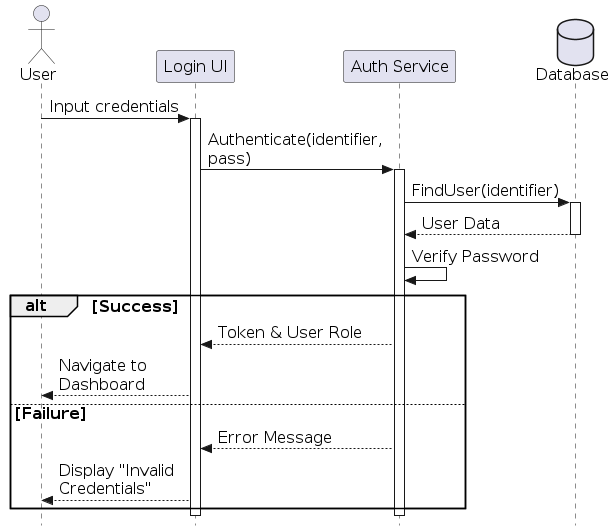
\includegraphics[width=0.8\textwidth]{Image/Diagrams/Sequence/LoginSequence.png}
  \vspace{1.0cm}
  \caption{Sequence diagram - Login}
\end{figure}
\newpage
\begin{figure}[H]
  \centering
   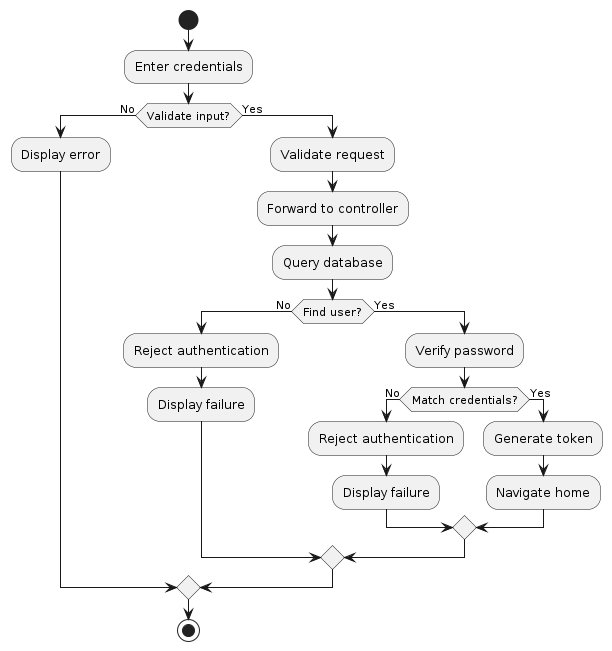
\includegraphics[width=0.9\textwidth]{Image/Diagrams/Activity/LoginActivity.png}
   \vspace{0.6cm}
  \caption{Activity diagram - Login}
\end{figure}

\newpage
\subsubsection{Đăng ký (Register)}
\begin{table}[H]
  \centering
  \renewcommand{\arraystretch}{1.3}
  \begin{tabular}{|l|p{0.75\textwidth}|}
    \hline
    \textbf{Usecase name} & Register \\ \hline
    \textbf{Actor} & End-user \\ \hline
    \textbf{Description} & Cho phép end-user tạo tài khoản mới để truy cập vào hệ thống. \\ \hline
    \textbf{Precondition} & End-user chưa có tài khoản trên hệ thống. \\ \hline
    \textbf{Postcondition} & Tài khoản mới được tạo thành công với vai trò được chọn và end-user có thể đăng nhập vào hệ thống. \\ \hline
    \textbf{Main flow} &
    1. End-user truy cập vào màn hình đăng ký. \newline
    2. Hệ thống hiển thị giao diện đăng ký. \newline
    3. Chọn vai trò (role): học sinh hoặc phụ huynh \newline
    4. End-user nhập username (đối với học sinh) hoặc email và họ tên (đối với phụ huynh), mật khẩu, xác nhận mật khẩu. \newline
    5. End-user nhấn nút Register. \newline
    7. Hệ thống xác thực dữ liệu đầu vào. \newline
    8. Hệ thống tạo tài khoản mới với vai trò đã chọn. \newline
    9. Hệ thống hiển thị thông báo đăng ký thành công. \\ \hline
    \textbf{Alternative flow} &
    \textit{Alternative flow 1: Quay về Landing Page} \newline
Bước 3: End-user nhấn vào "Quay lại". \newline
    Hệ thống chuyển hướng đến màn hình Landing Page. \\ \hline
    \textbf{Exception} &
    \textit{Exception 1: Dữ liệu không hợp lệ} \newline
    Tại bước 5: Hệ thống hiển thị thông báo lỗi validation và yêu cầu end-user nhập lại. \newline\newline
    \textit{Exception 2: User đã tồn tại} \newline
    Tại bước 6: Hệ thống kiểm tra và phát hiện username hoặc email đã được sử dụng, hiển thị thông báo lỗi và yêu cầu end-user nhập thông tin khác. \\ \hline
  \end{tabular}
  \caption{Usecase - Register}
  \label{table:uc_signup}
\end{table}
\newpage
\begin{figure}[H]
  \centering
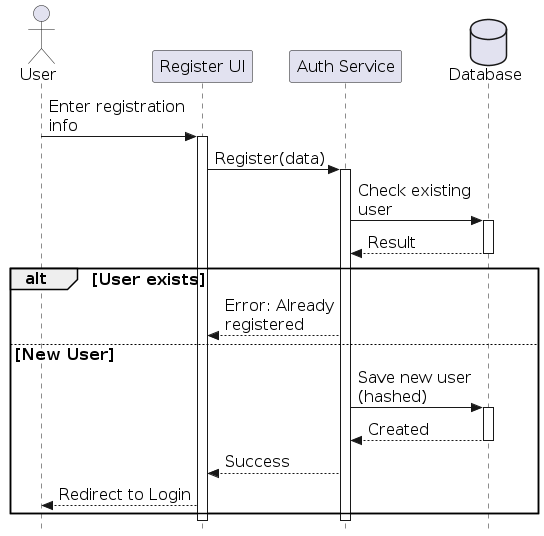
\includegraphics[width=0.8\textwidth]{Image/Diagrams/Sequence/RegisterSequence.png}
  \vspace{1.0cm}
  \caption{Sequence diagram - Register}
\end{figure}
\newpage
\begin{figure}[H]
  \centering
  \begin{adjustbox}{max height=0.9\textheight}
    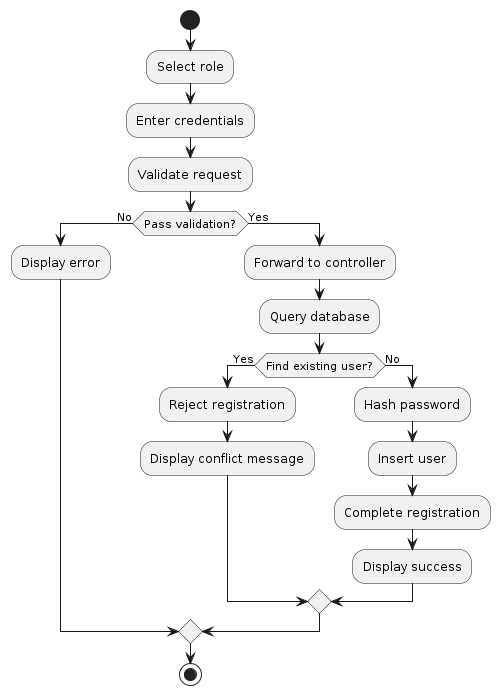
\includegraphics{Image/Diagrams/Activity/RegisterActivity.png}
  \end{adjustbox}
   \vspace{0.6cm}
  \caption{Activity diagram - Register}
\end{figure}
\newpage

\subsubsection{Làm bài tập (Do exercises)}
\begin{table}[H]
  \centering
  \renewcommand{\arraystretch}{1.3}
  \begin{tabular}{|l|p{0.75\textwidth}|}
    \hline
    \textbf{Usecase name} & Do Exercise \\ \hline

    \textbf{Actor} & Student \\ \hline

    \textbf{Description} & 
    Cho phép Student trả lời câu hỏi của bài tập, nhận kết quả đúng/sai, xem đáp án đúng và được hệ thống lưu lại lịch sử làm bài. \\ \hline

    \textbf{Precondition} & 
    Student đã đăng nhập và truy cập vào một bài tập hợp lệ. \\ \hline

    \textbf{Postcondition} & 
    Hệ thống ghi nhận kết quả làm bài, cập nhật điểm (nếu đúng), lưu lịch sử và hiển thị thông báo kết quả cho end-user. \\ \hline

    \textbf{Main flow} &
    1. Student mở bài tập trên màn hình làm bài. \newline
    2. Hệ thống hiển thị danh sách câu hỏi và giao diện trả lời. \newline
    3. Student chọn hoặc nhập câu trả lời cho một câu hỏi. \newline
    4. Student nhấn nút Submit. \newline
    5. Hệ thống kiểm tra tính hợp lệ của dữ liệu gửi lên. \newline
    6. Hệ thống so sánh câu trả lời của Student với đáp án đúng. \newline
    7. Hệ thống lưu kết quả vào lịch sử làm bài. \newline
    8. Nếu câu trả lời đúng, hệ thống cập nhật điểm thưởng. \newline
    9. Hệ thống trả về kết quả đúng/sai cho Student. \newline
    10. Student xem kết quả hiển thị trên màn hình. \\ \hline

    \textbf{Alternative flow} &
    \textit{Alternative flow 1: Xem đáp án đúng} \newline
    Sau bước 9: Student nhấn "View correct answer". \newline
    Hệ thống hiển thị đáp án đúng cho câu hỏi. \\ \hline

    \textbf{Exception} &
    \textit{Exception 1: Dữ liệu không hợp lệ} \newline
    Tại bước 5: Hệ thống trả về thông báo lỗi và yêu cầu Student kiểm tra lại dữ liệu. \newline\newline

    \textit{Exception 2: Câu trả lời sai} \newline
    Tại bước 6: Hệ thống trả về thông báo “Sai”, cho phép Student xem đáp án đúng. \\ \hline
  \end{tabular}
  \caption{Usecase - Do Exercise}
  \label{table:uc_acc02}
\end{table}
\newpage
\begin{figure}[H]
  \centering
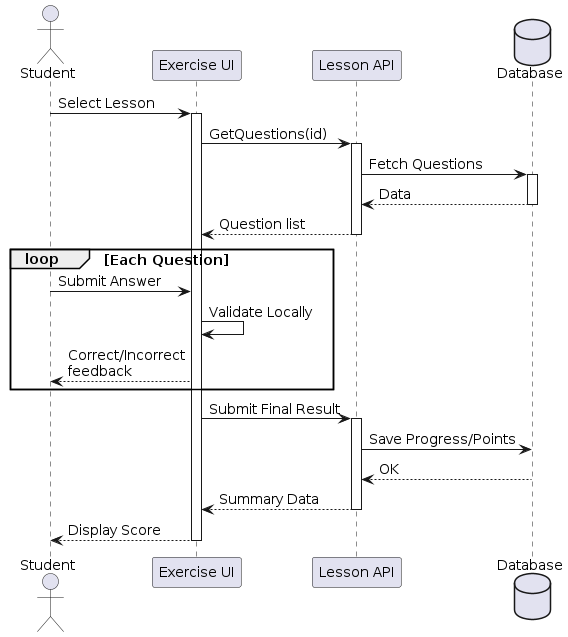
\includegraphics[width=0.8\textwidth]{Image/Diagrams/Sequence/DoExerciseSequence.png}
  \vspace{1.0cm}
  \caption{Sequence diagram - Do exercise}
\end{figure}
\newpage
\begin{figure}[H]
  \centering
  \begin{adjustbox}{max height=0.9\textheight}
    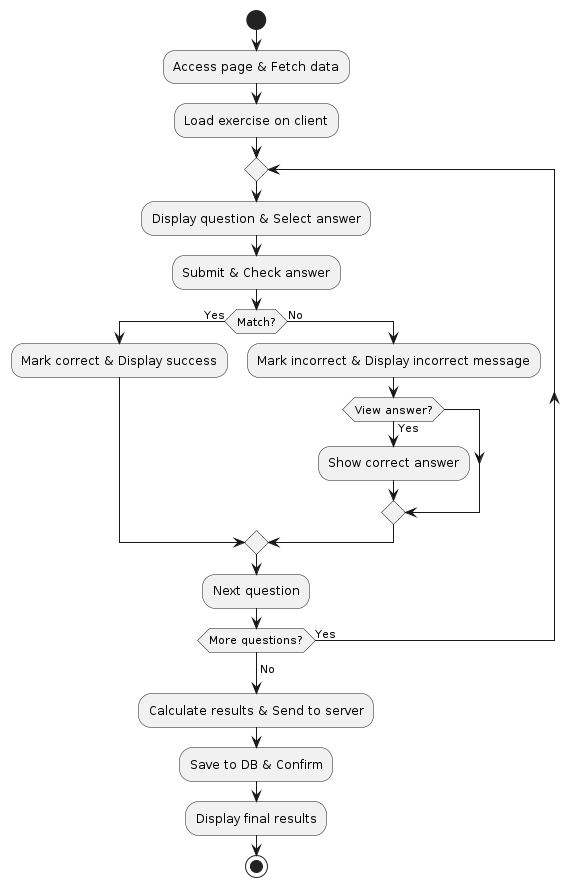
\includegraphics{Image/Diagrams/Activity/ExerciseActivity.png}
  \end{adjustbox}
   \vspace{0.6cm}
  \caption{Activity diagram - Do exercise}
\end{figure}

\subsubsection{Tham gia đấu trường (Join arena)}
\begin{table}[H]
\centering
\renewcommand{\arraystretch}{1.3}
\begin{tabular}{|l|p{0.75\textwidth}|}
\hline
\textbf{Usecase name} & Join Arena \\
\hline
\textbf{Actor} & Student \\
\hline
\textbf{Description} & Cho phép Student tham gia vào một arena để làm bài thi. \\
\hline
\textbf{Precondition} & Student đã đăng nhập vào hệ thống và có arena khả dụng. \\
\hline
\textbf{Postcondition} & Student hoàn thành bài thi arena và kết quả được lưu vào hệ thống. \\
\hline
\textbf{Main flow} & 
1. Student truy cập vào màn hình arena. \newline
2. Hệ thống lấy thông tin arena đang hoạt động (tuần hiện tại). \newline
3. Hệ thống kiểm tra trạng thái arena và trạng thái nộp bài của Student. \newline
4. Hệ thống hiển thị thông tin arena và thời gian còn lại. \newline
5. Student nhấn nút bắt đầu làm bài thi. \newline
6. Hệ thống tải câu hỏi (từ dễ đến khó). \newline
7. Hệ thống hiển thị các câu hỏi. \newline
8. Student trả lời các câu hỏi và nộp bài. \newline
9. Hệ thống validate yêu cầu nộp bài. \newline
10. Hệ thống kiểm tra trạng thái nộp bài. \newline
11. Hệ thống chấm điểm câu trả lời. \newline
12. Hệ thống tính điểm số và thời gian hoàn thành. \newline
13. Hệ thống lưu kết quả nộp bài (điểm, thời gian). \newline
14. Hệ thống cập nhật bảng xếp hạng. \newline
15. Hệ thống hiển thị điểm số và xếp hạng cho Student. \\
\hline
\textbf{Alternative flow} & 
\textit{Alternative flow 1: Arena đã hết hạn hoặc Student đã nộp bài} \newline
Tại bước 3: Hệ thống phát hiện arena đã hết hạn hoặc Student đã nộp bài trước đó. \newline
Hệ thống hiển thị thông báo "Arena đã đóng" hoặc "Đã nộp bài". \newline
Usecase kết thúc. \\
\hline
\textbf{Exception} & 
\textit{Exception 1: Dữ liệu nộp bài không hợp lệ} \newline
Tại bước 9: Hệ thống phát hiện dữ liệu yêu cầu không hợp lệ. \newline
Hệ thống hiển thị thông báo lỗi validation. \newline
Usecase kết thúc. \newline\newline
\textit{Exception 2: Student đã nộp bài trước đó} \newline
Tại bước 10: Hệ thống phát hiện Student đã nộp bài arena này trước đó. \newline
Hệ thống hiển thị thông báo "Đã nộp bài". \newline
Usecase kết thúc. \\
\hline
\end{tabular}
\caption{Usecase - Join Arena}
\label{table:uc_joinarena}
\end{table}

\newpage
\begin{figure}[H]
\centering
\begin{adjustbox}{max height=0.9\textheight}
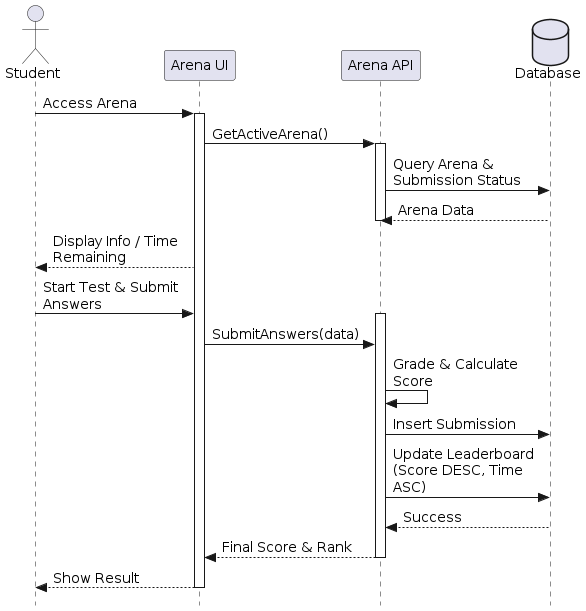
\includegraphics[width=0.8\textwidth]{Image/Diagrams/Sequence/ArenaSequence.png}
\end{adjustbox}
\vspace{1.0cm}
\caption{Sequence diagram - Join Arena}
\end{figure}

\newpage
\begin{figure}[H]
\centering
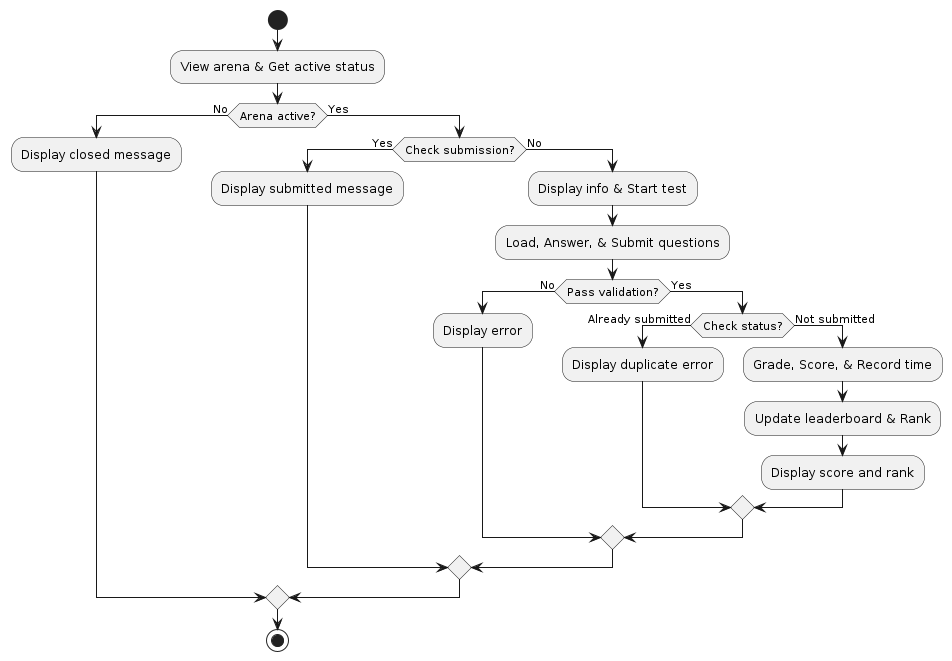
\includegraphics[width=0.9\textwidth]{Image/Diagrams/Activity/ArenaActivity.png}
\vspace{0.6cm}
\caption{Activity diagram - Join Arena}
\end{figure}

\subsubsection{Xem lịch sử làm bài (View exercise history)}
\begin{table}[H]
  \centering
  \renewcommand{\arraystretch}{1.3}
  \begin{tabular}{|l|p{0.75\textwidth}|}
    \hline
    \textbf{Usecase name} & View Exercise History \\ \hline
    \textbf{Actor} & Parent, Student \\ \hline
    \textbf{Description} & Cho phép Parent và Student xem lịch sử làm bài tập của Student. \\ \hline
    \textbf{Precondition} & Parent hoặc Student đã đăng nhập vào hệ thống. \\ \hline
    \textbf{Postcondition} & Lịch sử làm bài tập được hiển thị với các thông tin chi tiết. \\ \hline
    \textbf{Main flow} &
    1. Parent/Student truy cập vào màn hình lịch sử làm bài tập. \newline
    2. Hệ thống hiển thị các tùy chọn lọc (category, date range). \newline
    3. Parent/Student chọn bộ lọc và tìm kiếm. \newline
    4. Hệ thống truy vấn dữ liệu lịch sử làm bài tập. \newline
    5. Hệ thống hiển thị danh sách lịch sử (tên bài tập, ngày, điểm số, độ chính xác). \\ \hline
    \textbf{Alternative flow} &
    \textit{Alternative flow 1: Xem chi tiết bài tập} \newline
    Bước 5: Parent/Student nhấn vào một bài tập cụ thể. \newline
    Hệ thống truy vấn chi tiết các câu hỏi và câu trả lời. \newline
    Hệ thống hiển thị các câu hỏi với câu trả lời đúng/sai được đánh dấu. \\ \hline
    \textbf{Exception} &
    \textit{Exception 1: Không có dữ liệu lịch sử} \newline
    Tại bước 4: Hệ thống không tìm thấy dữ liệu lịch sử phù hợp với bộ lọc, hiển thị thông báo "Không có lịch sử làm bài tập". \\ \hline
  \end{tabular}
  \caption{Usecase - View Exercise History}
  \label{table:uc_viewhistory}
\end{table}
\newpage
\begin{figure}[H]
  \centering
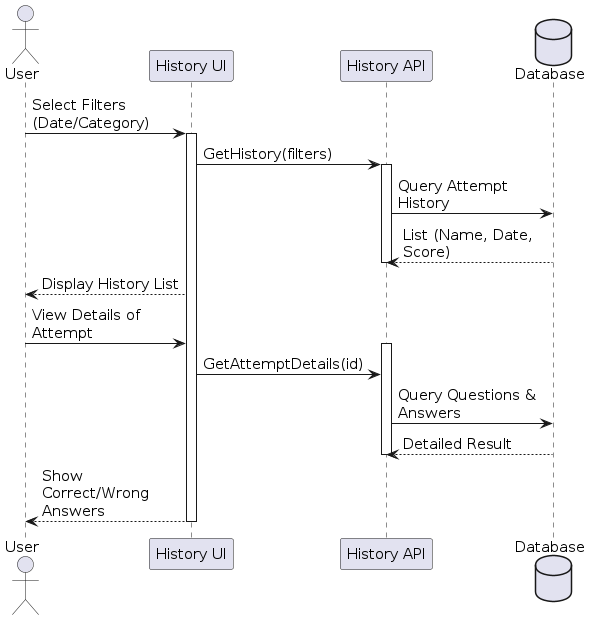
\includegraphics[width=\textwidth]{Image/Diagrams/Sequence/HistorySequence.png}
  \vspace{1.0cm}
  
  \caption{Sequence diagram - View Exercise History}
\end{figure}
\newpage
\begin{figure}[H]
  \centering
  \begin{adjustbox}{max height=0.9\textheight}
    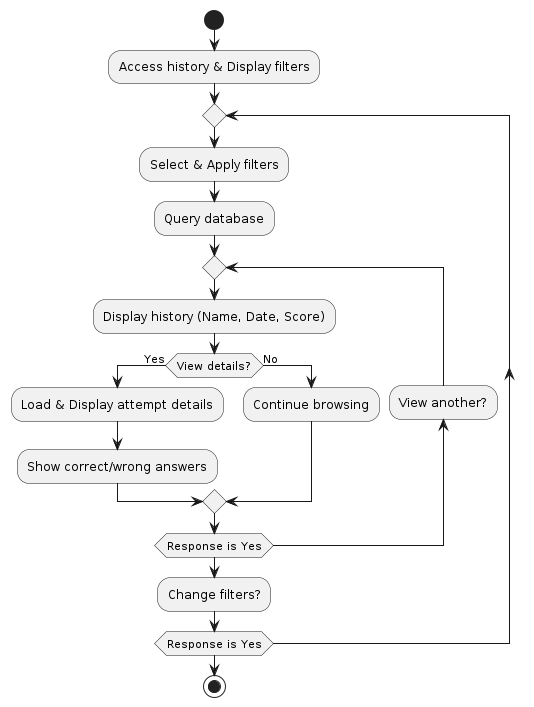
\includegraphics{Image/Diagrams/Activity/HistoryActivity.png}
  \end{adjustbox}
   \vspace{0.6cm}
  \caption{Activity diagram - View Exercise History}
\end{figure}
\newpage

\subsubsection{Chơi trò chơi (Play Minigames)}
\begin{table}[H]
\centering
\renewcommand{\arraystretch}{1.3}
\begin{tabular}{|l|p{0.75\textwidth}|}
\hline
\textbf{Usecase name} & Play Minigame \\
\hline
\textbf{Actor} & Student \\
\hline
\textbf{Description} & Cho phép Student chơi các minigame có sẵn trong hệ thống. \\
\hline
\textbf{Precondition} & Student đã đăng nhập vào hệ thống. \\
\hline
\textbf{Postcondition} & Student hoàn thành minigame và kết quả được lưu vào hệ thống. \\
\hline
\textbf{Main flow} & 
1. Student truy cập vào trang minigames. \newline
2. Hệ thống tải danh sách các minigame có sẵn. \newline
3. Hệ thống kiểm tra trạng thái premium của Student. \newline
4. Hệ thống hiển thị danh sách minigame (Free games + Premium games). \newline
5. Student chọn một minigame để chơi. \newline
6. Hệ thống kiểm tra quyền truy cập game. \newline
7. Hệ thống tải minigame. \newline
8. Hệ thống khởi động minigame. \newline
9. Student chơi minigame. \newline
10. Student hoàn thành và nộp kết quả minigame. \newline
11. Hệ thống lưu tiến trình và điểm số vào database. \newline
12. Hệ thống hiển thị kết quả hoàn thành/điểm số cho Student. \\
\hline
\textbf{Alternative flow} & 
\textit{Alternative flow 1: Student chọn chơi minigame khác} \newline
Tại bước 12: Student muốn chơi minigame khác. \newline
Student quay lại bước 4 để chọn minigame mới. \\
\hline
\textbf{Exception} & 
\textit{Exception 1: Không có quyền truy cập game premium} \newline
Tại bước 6: Hệ thống phát hiện Student không có quyền truy cập game premium. \newline
Hệ thống hiển thị thông báo "Yêu cầu Premium" với nút "Mua Premium". \newline
Usecase kết thúc. \newline\newline
\textit{Exception 2: Lỗi khi lưu kết quả} \newline
Tại bước 11: Hệ thống không thể lưu kết quả game. \newline
Hệ thống hiển thị thông báo lỗi. \newline
\\ \hline
\end{tabular}
\caption{Usecase - Play Minigame}
\label{table:uc_playminigame}
\end{table}

\newpage
\begin{figure}[H]
\centering
\begin{adjustbox}{max height=0.9\textheight}
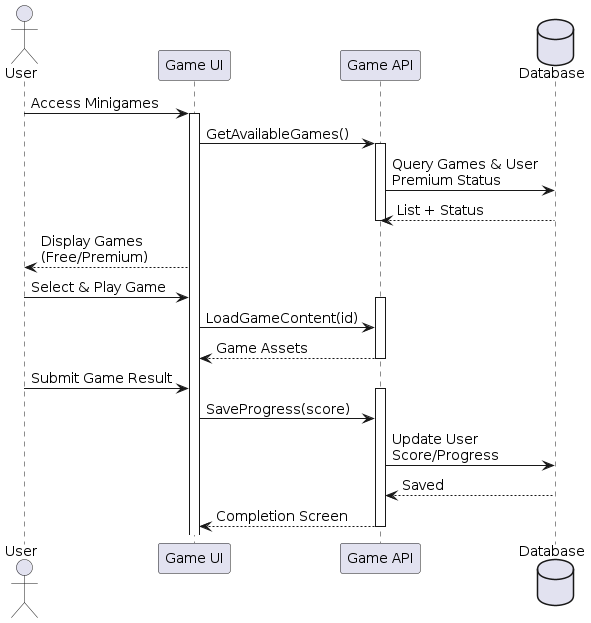
\includegraphics[width=0.8\textwidth]{Image/Diagrams/Sequence/GameSequence.png}
\end{adjustbox}
\vspace{1.0cm}
\caption{Sequence diagram - Play Minigame}
\end{figure}

\newpage
\begin{figure}[H]
\centering
\begin{adjustbox}{max height=0.9\textheight}
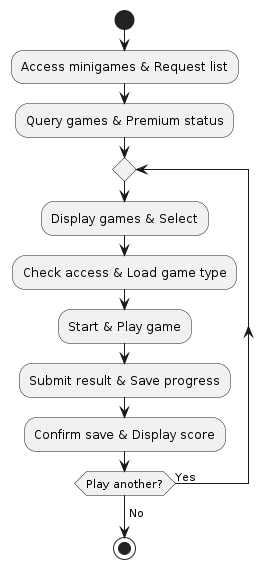
\includegraphics{Image/Diagrams/Activity/GameActivity.png}
\end{adjustbox}
\vspace{0.6cm}
\caption{Activity diagram - Play Minigame}
\end{figure}

\subsubsection{Xem thống kê của học sinh (View Student Statistics)}
\begin{table}[H]
\centering
\renewcommand{\arraystretch}{1.3}
\begin{tabular}{|l|p{0.75\textwidth}|}
\hline
\textbf{Usecase name} & View Student Statistics \\
\hline
\textbf{Actor} & Parent \\
\hline
\textbf{Description} & Cho phép Parent xem thống kê học tập và hoạt động của Student được liên kết. \\
\hline
\textbf{Precondition} & Parent đã đăng nhập vào hệ thống và có ít nhất một Student được liên kết. \\
\hline
\textbf{Postcondition} & Parent xem được thống kê chi tiết về hoạt động học tập và arena của Student. \\
\hline
\textbf{Main flow} & 
1. Parent truy cập vào trang thống kê. \newline
2. Hệ thống truy vấn danh sách Student liên kết với Parent. \newline
3. Hệ thống hiển thị dropdown chọn Student. \newline
4. Parent chọn một Student. \newline
5. Hệ thống truy vấn thống kê học tập (số bài tập đã làm, tỉ lệ làm đúng, số giờ hoạt động). \newline
6. Hệ thống truy vấn thống kê arena (xếp hạng, battle points, xếp hạng tuần, tỉ lệ làm đúng). \newline
7. Hệ thống truy vấn thành tích của Student (rank badge và tiến trình). \newline
8. Hệ thống hiển thị dashboard thống kê đầy đủ (Learning stats + Arena stats + Badge). \\
\hline
\textbf{Alternative flow} & 
\textit{Alternative flow 1: Áp dụng bộ lọc ngày tháng} \newline
Tại bước 8: Parent muốn xem thống kê theo khoảng thời gian cụ thể. \newline
Parent chọn khoảng ngày (From - To). \newline
Hệ thống truy vấn thống kê với bộ lọc ngày tháng. \newline
Hệ thống hiển thị kết quả thống kê đã lọc. \newline\newline
\textit{Alternative flow 2: Thay đổi Student} \newline
Tại bước 8: Parent muốn xem thống kê của Student khác. \newline
Parent chọn Student khác từ dropdown. \newline
Hệ thống quay lại bước 5 để tải thống kê của Student mới. \\
\hline
\textbf{Exception} & 
\textit{Exception 1: Khoảng ngày không hợp lệ} \newline
Tại Alternative flow 1: Hệ thống phát hiện khoảng ngày không hợp lệ. \newline
Hệ thống hiển thị thông báo lỗi "Invalid date range". \newline
Parent cần nhập lại khoảng ngày hợp lệ. \\
\hline
\end{tabular}
\caption{Usecase - View Student Statistics}
\label{table:uc_viewstudentstatistics}
\end{table}

\newpage
\begin{figure}[H]
\centering
\begin{adjustbox}{max height=0.9\textheight}
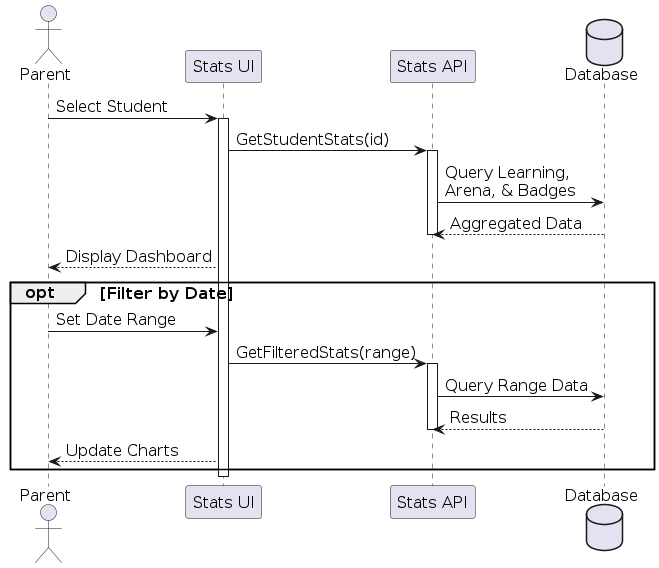
\includegraphics[width=0.8\textwidth]{Image/Diagrams/Sequence/StatsSequence.png}
\end{adjustbox}
\vspace{1.0cm}
\caption{Sequence diagram - View Student Statistics}
\end{figure}

\newpage
\begin{figure}[H]
\centering
\begin{adjustbox}{max height=0.9\textheight}
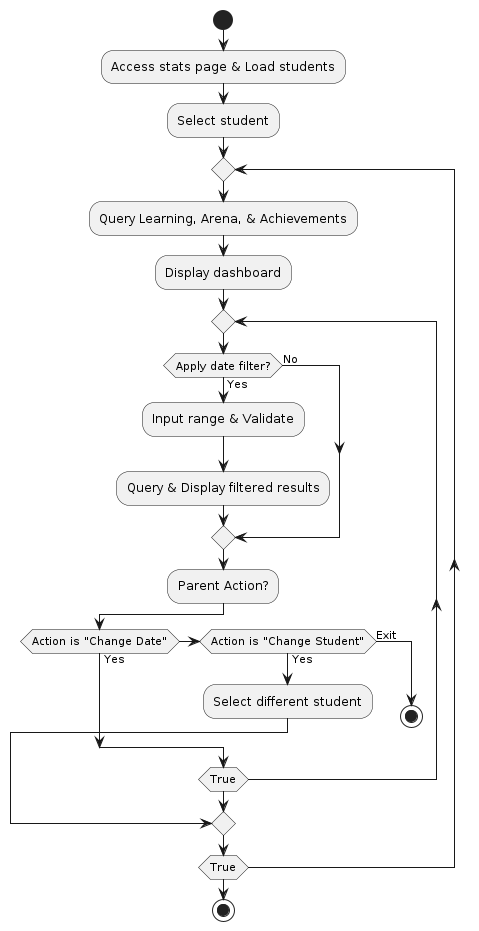
\includegraphics{Image/Diagrams/Activity/StatsActivity.png}
\end{adjustbox}
\vspace{0.6cm}
\caption{Activity diagram - View Student Statistics}
\end{figure}

\newpage
\subsubsection{Đăng ký gói Premium (Subscribe Premium)}
\begin{longtable}{|l|p{0.75\textwidth}|}
\caption{Usecase - Subscribe Premium}
\label{table:uc_subscribepremium} \\
\hline
\textbf{Usecase name} & Subscribe Premium \\
\hline
\textbf{Actor} & Parent \\
\hline
\textbf{Description} & Cho phép Parent nâng cấp tài khoản lên Premium để mở khóa toàn bộ tính năng cho Student. \\
\hline
\textbf{Precondition} & Parent đã đăng nhập vào hệ thống. \\
\hline
\textbf{Postcondition} & Parent nâng cấp thành công tài khoản Premium và tất cả tính năng được kích hoạt cho Student. \\
\hline
\textbf{Main flow} & 
1. Parent truy cập vào trang premium subscription. \newline
2. Hệ thống truy vấn các gói đăng ký có sẵn. \newline
3. Hệ thống truy vấn trạng thái đăng ký hiện tại của Parent. \newline
4. Hệ thống hiển thị các gói đăng ký (Free: 0đ vs Premium: 599,000đ). \newline
5. Parent chọn gói Premium. \newline
6. Hệ thống hiển thị các lợi ích của Premium (No time limit, No minigames limit, All features unlocked). \newline
7. Parent nhấn nút "Nâng cấp ngay". \newline
8. Hệ thống tạo đơn hàng đăng ký. \newline
9. Hệ thống khởi tạo phiên thanh toán. \newline
10. Hệ thống hiển thị các phương thức thanh toán (Bank transfer, QR code, E-wallet). \newline
11. Parent hoàn thành thanh toán. \newline
12. Payment Gateway gửi thông báo webhook về kết quả thanh toán. \newline
13. Hệ thống xác minh giao dịch thanh toán. \newline
14. Hệ thống cập nhật đăng ký Parent lên Premium. \newline
15. Hệ thống kích hoạt các tính năng premium (Unlock minigames, Remove time limits, Grant full access). \newline
16. Hệ thống cập nhật trạng thái đơn hàng thành "completed". \newline
17. Hệ thống gửi thông báo xác nhận cho Parent. \newline
18. Hệ thống hiển thị thông báo "Nâng cấp thành công!". \newline
19. Hệ thống chuyển hướng Parent về dashboard. \\
\hline
\textbf{Alternative flow} & 
\textit{Alternative flow 1: Parent xem trạng thái đăng ký hiện tại} \newline
Tại bước 4: Parent muốn xem thông tin đăng ký hiện tại. \newline
Parent nhấn "View current plan". \newline
Hệ thống truy vấn chi tiết đăng ký của Parent. \newline
Hệ thống hiển thị gói hiện tại và ngày hết hạn. \newline
Parent quay lại bước 4. \newline\newline
\textit{Alternative flow 2: Parent hủy thanh toán} \newline
Tại bước 11: Parent quyết định không thanh toán. \newline
Parent đóng trang thanh toán. \newline
Usecase kết thúc. \\
\hline
\textbf{Exception} &
\textit{Exception 1: Thanh toán thất bại} \newline
Tại bước 12: Payment Gateway thông báo thanh toán thất bại. \newline
Hệ thống cập nhật trạng thái đơn hàng thành "failed". \newline
Hệ thống hiển thị thông báo lỗi thanh toán với tùy chọn thử lại. \newline
Parent có thể quay lại bước 10 để thử lại thanh toán hoặc kết thúc usecase. \newline\newline
\textit{Exception 2: Lỗi xác minh giao dịch} \newline
Tại bước 13: Hệ thống không thể xác minh giao dịch. \newline
Hệ thống ghi log lỗi và thông báo cho admin. \newline
Hệ thống hiển thị thông báo "Đang xử lý, vui lòng chờ xác nhận". \newline
Usecase kết thúc. \\
\hline
\end{longtable}


\newpage
\begin{figure}[H]
\centering
\begin{adjustbox}{max height=0.9\textheight}
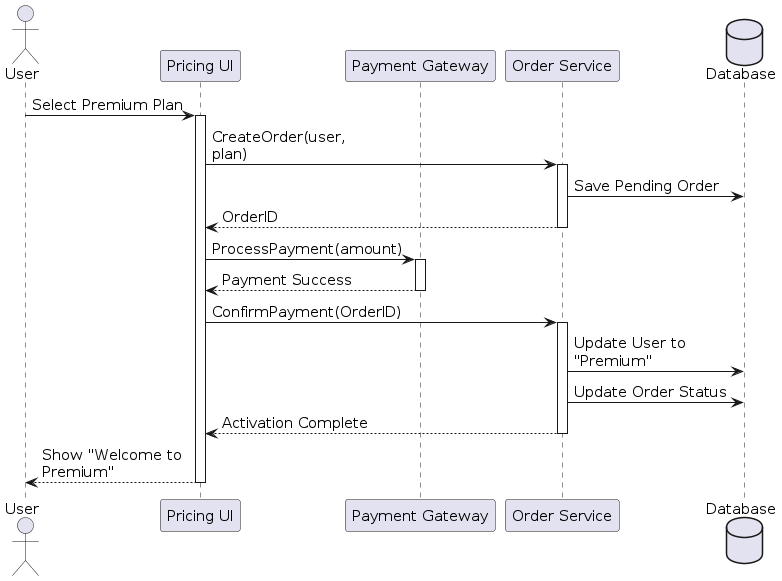
\includegraphics[width=0.9\textwidth]{Image/Diagrams/Sequence/PurchaseSequence.png}
\end{adjustbox}
\vspace{1.0cm}
\vspace{1.0em}
\caption{Sequence diagram - Subscribe Premium}
\end{figure}

\newpage
\begin{figure}[H]
\centering
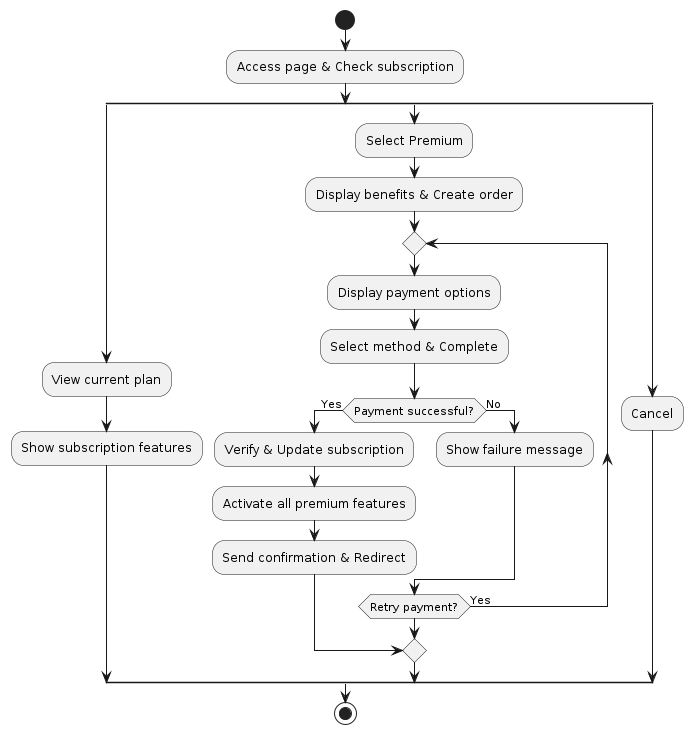
\includegraphics[width=0.9\textwidth]{Image/Diagrams/Activity/PurchaseActivity.png}
\vspace{0.6cm}
\caption{Activity diagram - Subscribe Premium}
\end{figure}

\newpage
\subsubsection{Quản lý bài học (Manage Lesson)}
\begin{longtable}{|l|p{0.75\textwidth}|}
	\caption{Usecase - Manage Lesson}
	\label{table:uc_managelesson} \\
	\hline
	\textbf{Usecase name} & Manage Lesson\\
	\hline
	\endfirsthead
	\hline
	\textbf{Usecase name} & Manage Lesson (tiếp) \\
	\hline
	\endhead
	\hline
	\textbf{Actor} & Admin \\
	\hline
	\textbf{Description} & Cho phép Admin quản lý chi tiết một bài học cụ thể, bao gồm việc thêm mới bài học (thủ công/Excel), chỉnh sửa nội dung lý thuyết bằng HTML và quản lý danh sách bài tập bằng giao diện Form hoặc mã nguồn JSON. \\
	\hline
	\textbf{Precondition} & Admin đã truy cập vào giao diện Quản lý bài học. \\
	\hline
	\textbf{Postcondition} & Các thay đổi về nội dung lý thuyết và bài tập được lưu trữ thành công vào hệ thống. \\
	\hline
	\textbf{Main flow} &
	1. Admin chọn phương thức khởi tạo bài học: nhập Form thủ công hoặc tải tệp Excel. \newline
	2. Hệ thống hiển thị giao diện chi tiết bài học sau khi khởi tạo thành công. \newline
	3. Admin truy cập tab "Quản lý lý thuyết" để chỉnh sửa các khối nội dung HTML. \newline
	4. Admin truy cập tab "Quản lý bài tập" để thêm, sửa hoặc xóa các câu hỏi. \newline
	5. Hệ thống thực hiện kiểm tra tính hợp lệ của dữ liệu (Validation) và cú pháp (JSON/HTML). \newline
	6. Admin nhấn "Lưu thay đổi". \newline
	7. Hệ thống hiển thị thông báo thành công và cập nhật lại trạng thái bài học. \\
	\hline
	\textbf{Alternative flow} &
	\textit{Alternative flow 1: Import bài tập/bài học từ Excel} \newline
	Tại bước 1: Admin chọn "Import Excel" và tải tệp lên. \newline
	Hệ thống kiểm tra cấu trúc tệp; nếu hợp lệ, dữ liệu sẽ được đổ vào các trường tương ứng. \newline\newline
	\textit{Alternative flow 2: Quản lý bài tập bằng JSON} \newline
	Tại bước 4: Admin chuyển đổi chế độ nhập liệu từ Form sang "JSON Editor". \newline
	Admin chỉnh sửa trực tiếp mã JSON của danh sách bài tập. \newline
	Hệ thống kiểm tra lỗi cú pháp JSON thời gian thực. \newline\newline
	\textit{Alternative flow 3: Preview nội dung} \newline
	Tại bất kỳ bước nào trước khi lưu: Admin nhấn nút "Preview". \newline
	Hệ thống hiển thị giao diện bài học thực tế (Live View) như cách học sinh sẽ nhìn thấy. \newline\newline
	\textit{Alternative flow 4: Xuất tệp mẫu (Export Sample)} \newline
	Tại giao diện quản lý: Admin nhấn "Tải tệp mẫu". \newline
	Hệ thống tạo và tải xuống tệp Excel trống có sẵn định dạng cột chuẩn. \\
	\hline
	\textbf{Exception} &
	\textit{Exception 1: Lỗi cú pháp mã nguồn (JSON/HTML)} \newline
	Tại bước 5: Hệ thống phát hiện lỗi cú pháp trong trình chỉnh sửa. \newline
	Hệ thống đánh dấu đỏ vị trí lỗi và vô hiệu hóa nút "Lưu". \newline\newline
	\textit{Exception 2: Tệp Excel không hợp lệ} \newline
	Tại AF1: Tệp tải lên sai định dạng hoặc chứa dữ liệu rác. \newline
	Hệ thống từ chối nhập liệu. \newline\newline
	\textit{Exception 3: Trùng lặp mã bài học} \newline
	Tại bước 6: Admin lưu bài học với mã định danh đã tồn tại. \newline
	Hệ thống báo lỗi "Mã bài học đã tồn tại" và yêu cầu nhập lại. \\
	\hline
\end{longtable}

\newpage
\begin{figure}[H]
\centering
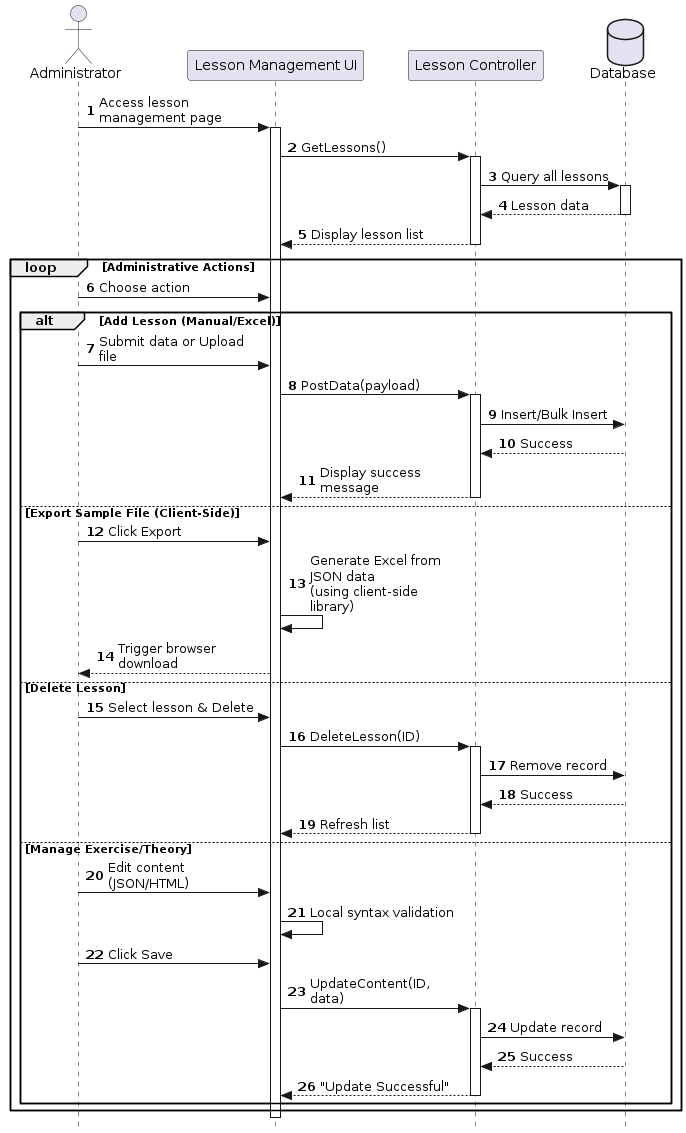
\includegraphics[width=0.9\textwidth]{Image/Diagrams/Sequence/AdminSequence.png}
\vspace{0.5cm}
\caption{Sequence diagram - Manage Lesson}
\end{figure}

\newpage
\begin{figure}[H]
\centering
\begin{adjustbox}{max width=\textwidth, max height=0.9\textheight}
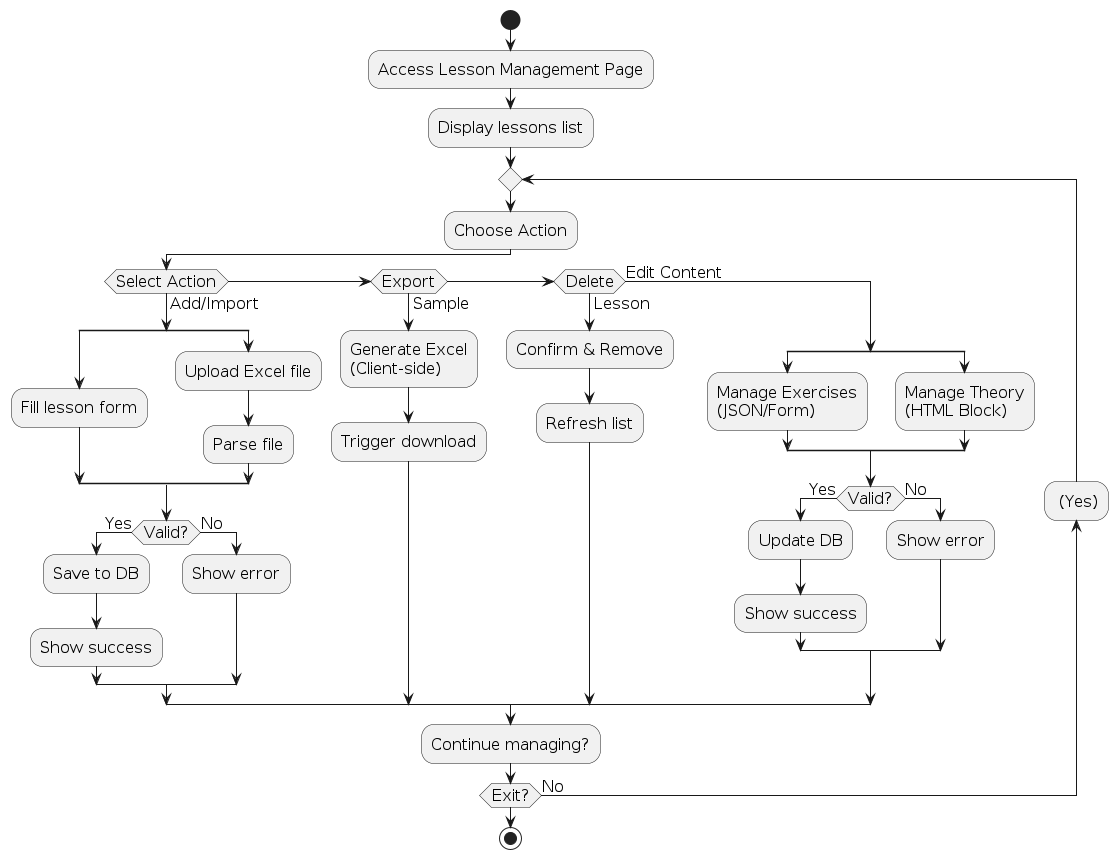
\includegraphics{Image/Diagrams/Activity/AdminActivity.png}
\end{adjustbox}
\vspace{0.6cm}
\caption{Activity diagram - Manage Lesson}
\end{figure}

\newpage
\subsection{Mô tả kiến trúc hệ thống}
\begin{figure}[h!]
	\centering
	\setlength{\abovecaptionskip}{10pt}
	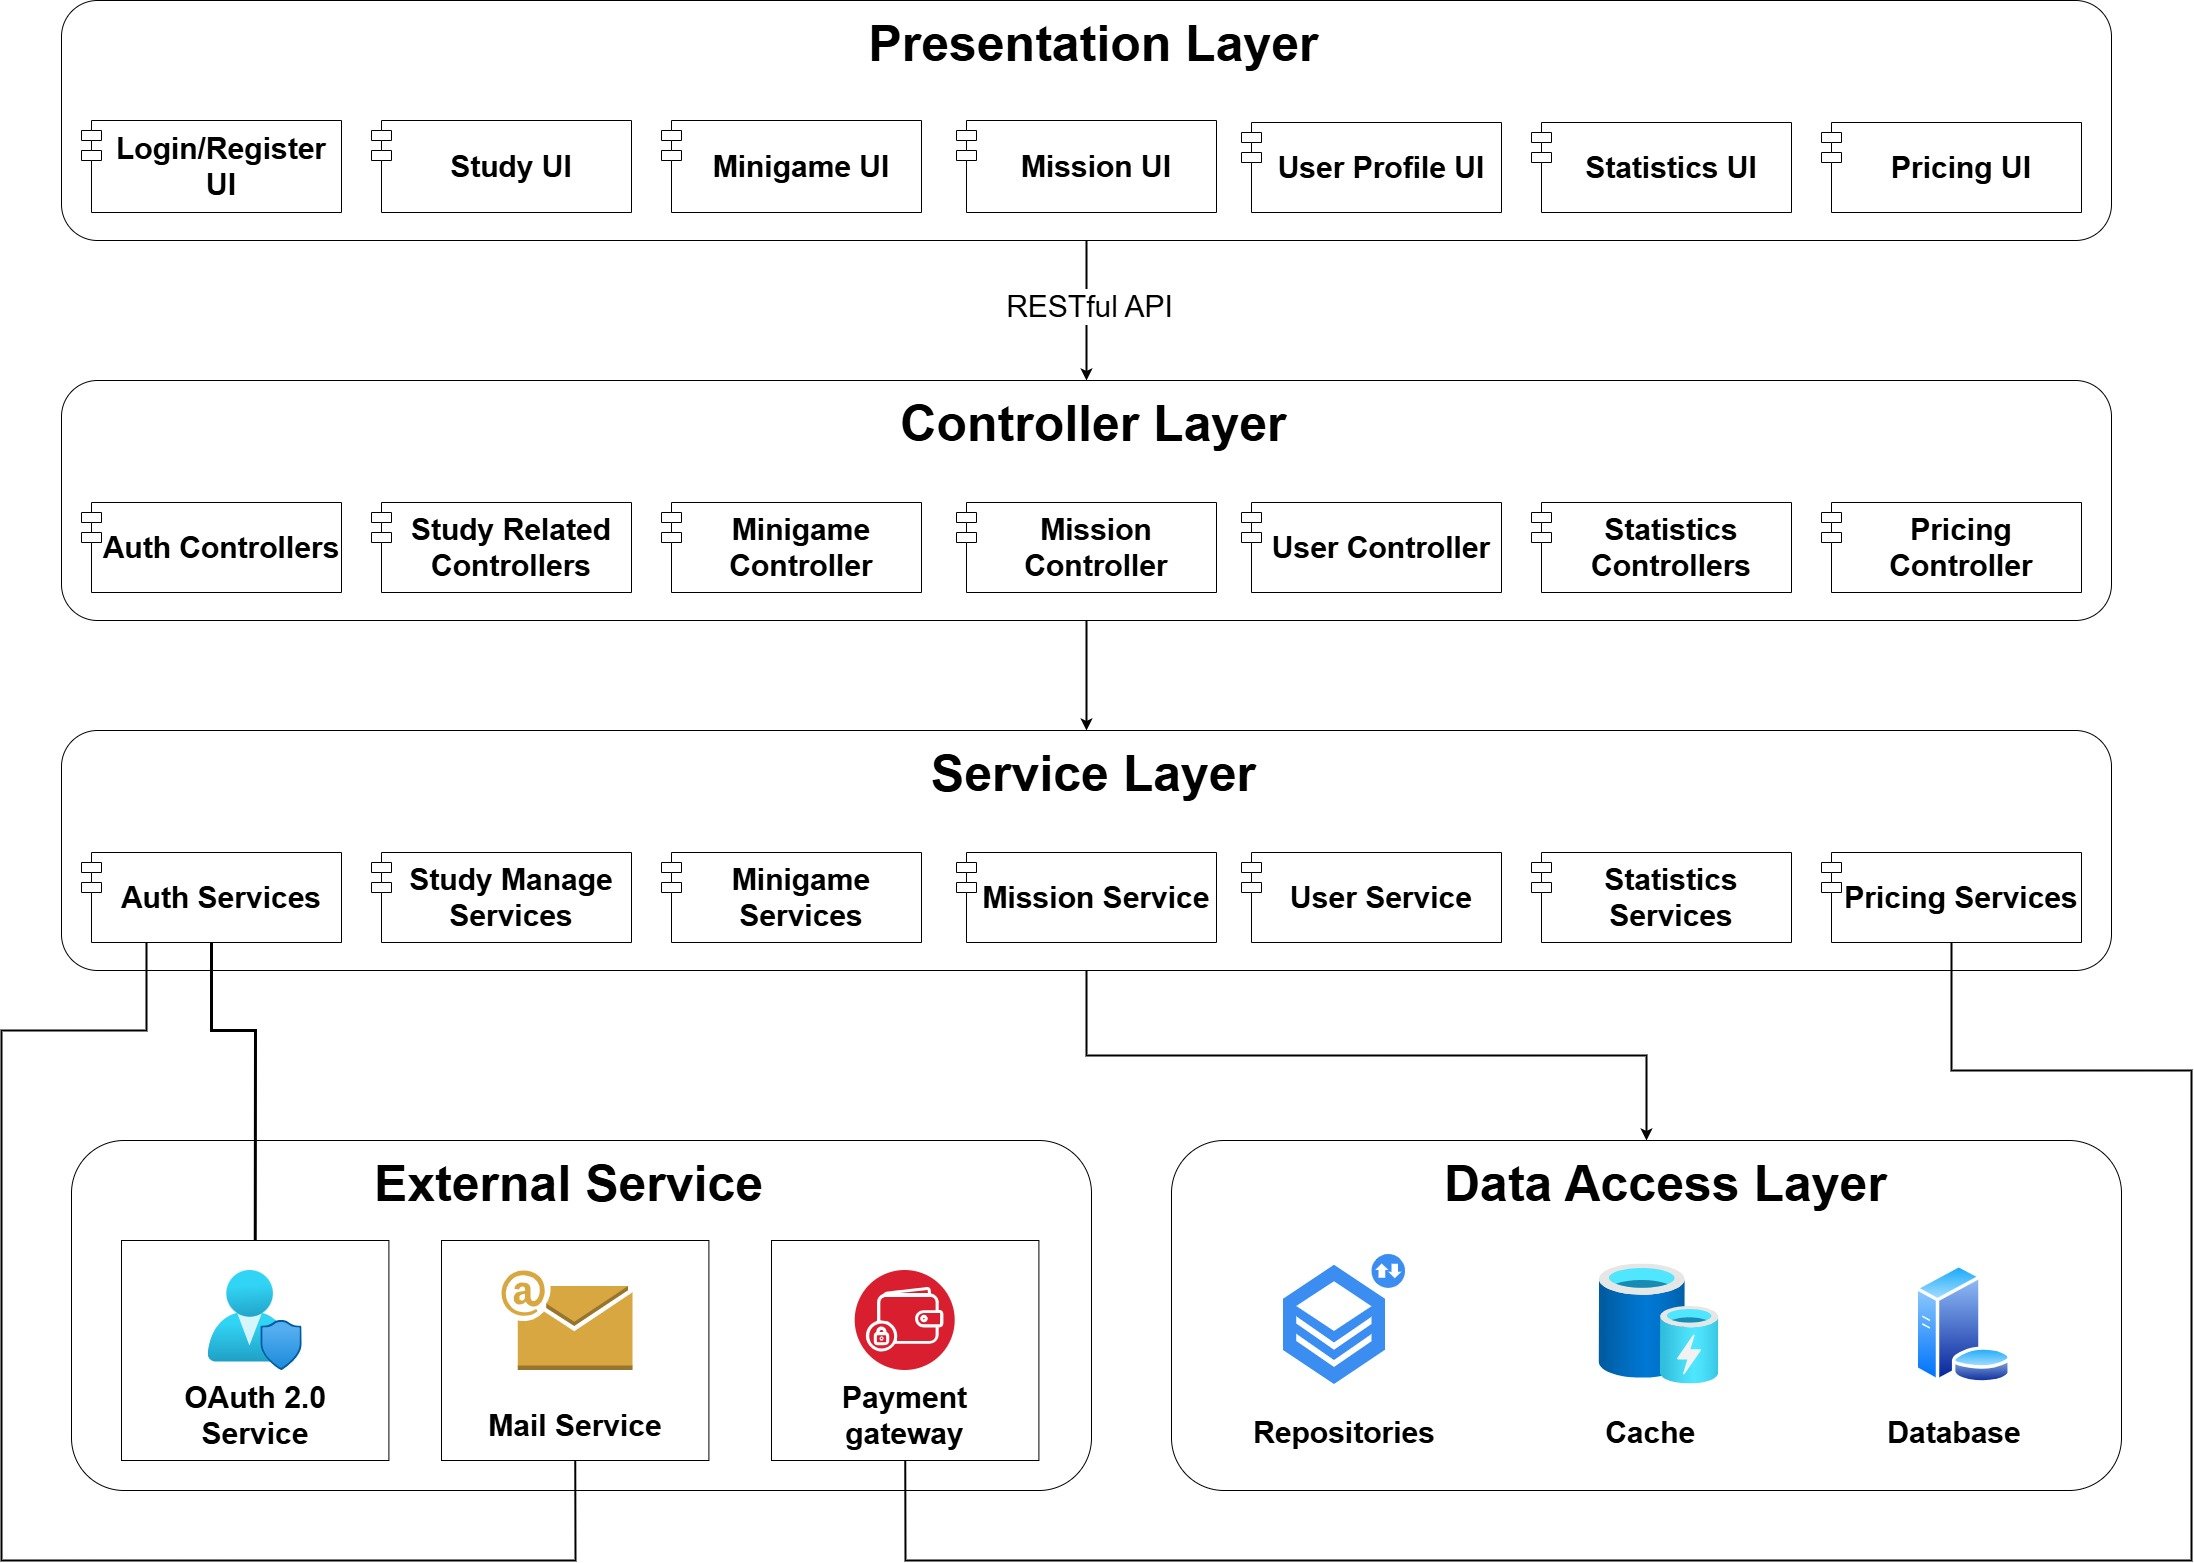
\includegraphics[width=\textwidth]{Image/Architecture.jpg}
	\caption{Sơ đồ kiến trúc tổng thể của hệ thống}
	\label{fig:system-architecture}
\end{figure}


Hệ thống được thiết kế theo mô hình kiến trúc nhiều tầng (layered architecture), nhằm tách biệt rõ ràng giữa giao diện người dùng, xử lý nghiệp vụ và truy cập dữ liệu, từ đó tăng khả năng mở rộng, bảo trì và kiểm thử.
Hệ thống được thiết kế theo mô hình kiến trúc nhiều tầng (layered architecture), nhằm tách biệt rõ ràng giữa giao diện người dùng, xử lý nghiệp vụ và truy cập dữ liệu, từ đó tăng khả năng mở rộng, bảo trì và kiểm thử.

\subsubsection{Tầng Trình bày (Presentation Layer)}
Tầng trình bày chịu trách nhiệm tương tác trực tiếp với người dùng, bao gồm các giao diện và chức năng như:
\begin{itemize}
	\item \textit{Đăng nhập/Đăng ký} (Login/Register UI)
	\item Các giao diện liên quan đến học tập: Chủ đề, Đấu trường, Bài kiểm tra, Bài tập tương tác được thể hiện chung trên sơ đồ \textit{Hình \ref{fig:system-architecture} } qua component Study UI.
	\item \textit{Nhiệm vụ} (Mission UI)
	\item \textit{Hồ sơ người dùng} (User Profile UI)
	\item \textit{Trò chơi} (Minigame UI)
	\item \textit{Thống kê} (Statistics UI): bao gồm các giao diện lịch sử, bảng xếp hạng, các thông số học tập,...
\end{itemize}

Các thành phần thuộc tầng này không xử lý logic nghiệp vụ, mà chỉ có nhiệm vụ gửi yêu cầu (request) đến Tầng Điều khiển và hiển thị kết quả (response) trả về cho người dùng.

\subsubsection{Tầng Điều khiển (Controller Layer)}
Tầng điều khiển đóng vai trò trung gian giữa Tầng Trình bày và Tầng Dịch vụ (Service Layer).  

Mỗi bộ điều khiển (Controller) như: \textit{Xác thực} (Auth), \textit{Trò chơi} (Minigame), \textit{Nhiệm vụ} (Mission), \textit{Học tập} (Study), \textit{Thống kê} (Statistics),... tiếp nhận yêu cầu từ giao diện người dùng, điều phối luồng xử lý và gọi các thành phần nghiệp vụ tương ứng.  

\subsubsection{Tầng Dịch vụ (Service Layer)}
Tầng Dịch vụ chứa các dịch vụ cốt lõi (Core Services) của hệ thống, bao gồm \textit{Dịch vụ Xác thực} (Auth Service), \textit{Dịch vụ Trò chơi} (Minigame Service), \textit{Các dịch vụ liên quan đến học tập} (Study Services), \textit{Dịch vụ Nhiệm vụ} (Mission Service), \textit{Dịch vụ quản lý người dùng} (User Service), \textit{Các dịch vụ Thống kê} (Statistics Services), \textit{Các dịch vụ liên quan đến gói trả phí và thanh toán} (Pricing Services).  

Mỗi dịch vụ chịu trách nhiệm xử lý một nhóm nghiệp vụ cụ thể, đóng gói các quy tắc nghiệp vụ và đảm bảo tính nhất quán của dữ liệu.  
Các dịch vụ có thể giao tiếp với nhau khi cần thiết, đồng thời tương tác với các dịch vụ bên ngoài.

\subsubsection{Tầng Truy cập Dữ liệu (Data Access Layer)}
Tầng truy cập dữ liệu chịu trách nhiệm lưu trữ và truy xuất dữ liệu từ hệ quản trị cơ sở dữ liệu MongoDB.  

Mọi thao tác liên quan đến dữ liệu đều được thực hiện thông qua tầng này, giúp cô lập logic nghiệp vụ khỏi chi tiết cài đặt của hệ quản trị cơ sở dữ liệu.

\subsubsection{Các Dịch vụ Bên ngoài (External Services)}
Hệ thống tích hợp với các dịch vụ bên ngoài như \textit{Cổng thanh toán} (Payment Gateway) để xử lý giao dịch, \textit{Dịch vụ Email} (Email Service) để gửi thông báo, dịch vụ xác thực người dùng thông qua tài khoản Google.  

Việc tách riêng các dịch vụ bên ngoài giúp hệ thống dễ dàng thay thế, mở rộng hoặc nâng cấp trong tương lai mà không ảnh hưởng đến các thành phần cốt lõi.

\subsubsection{Luồng Xử lý Tổng quát}
Người dùng tương tác với Tầng Trình bày, các yêu cầu được chuyển đến bộ điều khiển (Controller) tương ứng.  
Sau khi dữ liệu được xác thực và kiểm tra hợp lệ, yêu cầu sẽ được xử lý tại Tầng Dịch vụ thông qua các dịch vụ phù hợp, đồng thời truy xuất hoặc cập nhật dữ liệu tại Tầng Truy cập Dữ liệu.  
Cuối cùng, kết quả xử lý được trả về Tầng Trình bày để hiển thị cho người dùng.

\subsection{Thiết kế cơ sở dữ liệu}
Phần này trình bày chi tiết các thực thể chính trong hệ thống Dino Math, bao gồm vai trò, đặc điểm và mối quan hệ giữa chúng. Các thực thể được thiết kế nhằm đáp ứng đồng thời hai mục tiêu cốt lõi:
\begin{enumerate}
	\item Quản lý hiệu quả quá trình học tập của người dùng.
	\item Tích hợp các yếu tố trò chơi hóa để nâng cao mức độ tương tác và hứng thú học tập.
\end{enumerate}
\begin{figure}[H]
	\centering
	\includegraphics[width=\textwidth]{Image/ERD.jpg}
	\vspace{0.5cm}
	
	\caption{Sơ đồ thực thể – quan hệ (ERD) của hệ thống}
	\label{fig:erd-diagram}
\end{figure}

Dựa trên sơ đồ thực thể – quan hệ (ERD) ở Hình~\ref{fig:erd-diagram}, hệ thống được chia thành các thực thể chính sau đây.

\subsubsection{Quản lý Người dùng và Gia đình (User \& Family)}

Đây là nhóm thực thể nền tảng, đóng vai trò trung tâm trong việc quản lý tài khoản, phân quyền truy cập và mối quan hệ giữa các người dùng trong hệ thống.

\subsubsubsection{User (Người dùng)}

\texttt{User} là thực thể trung tâm của hệ thống, đại diện cho tất cả các đối tượng sử dụng ứng dụng, bao gồm học sinh, phụ huynh và quản trị viên. 
Mỗi người dùng được phân loại thông qua thuộc tính \texttt{role} và được kiểm soát trạng thái hoạt động thông qua \texttt{status}.

\newline
\vspace{0.2cm}
Thực thể \texttt{User} lưu trữ các thông tin cá nhân cơ bản như tên, email, mật khẩu (đã được mã hóa), ảnh đại diện và các thiết lập cá nhân hóa trải nghiệm (ngôn ngữ, thông báo, v.v.). 
Bên cạnh đó, \texttt{User} còn giữ vai trò liên kết tới hầu hết các chức năng nghiệp vụ quan trọng trong hệ thống.

\begin{table}[H]
	\centering
	\begin{tabularx}{\textwidth}{|l|l|X|}
		\hline
		\textbf{Thuộc tính} & \textbf{Kiểu dữ liệu} & \textbf{Mô tả} \\ \hline
		\_id & ObjectId & Khóa chính định danh người dùng. \\ \hline
		name & String & Họ và tên hiển thị. \\ \hline
		username & String & Tên đăng nhập. \\ \hline
		email & String & Địa chỉ email liên kết tài khoản. \\ \hline
		password & String & Mật khẩu (đã được mã hóa). \\ \hline
		role & Enum & Vai trò: \texttt{student}, \texttt{parent}, \texttt{admin}. \\ \hline
		status & Enum & Trạng thái: \texttt{active}, \texttt{inactive}, \texttt{pending\_profile}. \\ \hline
		familyId & ObjectId & Tham chiếu đến gia đình (Family). \\ \hline
		gradeId & ObjectId & Tham chiếu đến khối lớp (Grade). \\ \hline
		quartz & Number & Số lượng đá quý hiện có. \\ \hline
		battlePoints & Number & Điểm thi đấu tích lũy. \\ \hline
		rankId & ObjectId & Tham chiếu đến cấp bậc (Rank). \\ \hline
	\end{tabularx}
	\caption{Các thuộc tính chính của thực thể User}
\end{table}
\newline
\textbf{Các mối quan hệ chính của User:}
\begin{itemize}
	\item Thuộc về một \texttt{Family}, cho phép liên kết giữa phụ huynh và học sinh.
	\item Được gán vào một \texttt{Grade} để xác định chương trình học phù hợp.
	\item Liên kết với một \texttt{Rank} nhằm phản ánh cấp bậc và tiến trình của người dùng trong hệ thống.
	\item Có nhiều bản ghi \texttt{Progress} để theo dõi tiến độ học tập.
	\item Tham gia các bài giảng và bài kiểm tra, sinh ra các thực thể \texttt{LectureResult}, \texttt{ExerciseResult} và \texttt{AssessmentResult}.
	\item Tham gia các hoạt động thi đấu thông qua \texttt{Participation} trong các \texttt{Arena}.
	\item Nhận phần thưởng và thành tựu thông qua các thực thể \texttt{Achievement} và \texttt{RewardRecord}.
\end{itemize}

\subsubsubsection{Family (Gia đình)}
\texttt{Family} đại diện cho một nhóm người dùng có mối quan hệ gia đình, cho phép phụ huynh quản lý và theo dõi quá trình học tập của học sinh. 
Mỗi gia đình được tạo ra với một mã mời (\texttt{inviteCode}), cho phép các thành viên mới tham gia một cách thuận tiện.

\begin{table}[H]
	\centering
	\begin{tabularx}{\textwidth}{|l|l|X|}
		\hline
		\textbf{Thuộc tính} & \textbf{Kiểu dữ liệu} & \textbf{Mô tả} \\ \hline
		\_id & ObjectId & Khóa chính định danh gia đình. \\ \hline
		name & String & Tên nhóm gia đình. \\ \hline
		inviteCode & String & Mã mời thành viên mới. \\ \hline
		inviteSingleUse & Boolean & Xác định mã mời dùng một lần hay nhiều lần. \\ \hline
	\end{tabularx}
	\caption{Các thuộc tính chính của thực thể Family}
\end{table}

\newline
\textbf{Các mối quan hệ chính của Family:}
\begin{itemize}
	\item Chứa nhiều thành viên \texttt{User}.
	\item Liên kết với các báo cáo học tập tổng hợp thông qua \texttt{FamilyReport}.
	\item Tổ chức các hoạt động tương tác thông qua các \texttt{FamilyGame}.
\end{itemize}

\subsubsection{Cấu trúc Chương trình Học (Academic \& Structure)}
Nhóm thực thể này chịu trách nhiệm tổ chức nội dung học tập theo chương trình giáo dục, đồng thời hỗ trợ hiển thị và điều hướng nội dung một cách trực quan trong hệ thống.

\subsubsubsection{Grade (Khối lớp)}

\texttt{Grade} đại diện cho một cấp độ học tập cụ thể (ví dụ: Lớp 1, Lớp 2). 
Mỗi khối lớp được liên kết với một \texttt{World} riêng biệt, giúp xây dựng chủ đề và giao diện học tập phù hợp với từng độ tuổi.

\begin{table}[H]
	\centering
	\begin{tabularx}{\textwidth}{|l|l|X|}
		\hline
		\textbf{Thuộc tính} & \textbf{Kiểu dữ liệu} & \textbf{Mô tả} \\ \hline
		\_id & ObjectId & Khóa chính định danh khối lớp. \\ \hline
		name & String & Tên khối lớp (ví dụ: Lớp 1). \\ \hline
		level & Number & Cấp độ số của khối lớp. \\ \hline
		worldId & ObjectId & Tham chiếu đến thế giới (World) tương ứng. \\ \hline
	\end{tabularx}
	\caption{Các thuộc tính chính của thực thể Grade}
\end{table}

\newline
\textbf{Các mối quan hệ chính của Grade:}
\begin{itemize}
	\item Liên kết một--một với \texttt{World}.
	\item Chứa nhiều \texttt{Topic} thuộc chương trình học của khối lớp.
	\item Có nhiều \texttt{User} đang theo học.
	\item Liên quan đến các bài kiểm tra \texttt{Assessment}.
\end{itemize}

\subsubsubsection{AcademicTerm (Học kỳ)}
\texttt{AcademicTerm} được sử dụng để phân chia chương trình học theo từng giai đoạn thời gian như Học kỳ I, Học kỳ II hoặc Học kỳ hè. 
Thực thể này giúp hệ thống hiển thị và quản lý nội dung học tập phù hợp với mốc thời gian thực tế.
\begin{table}[H]
	\centering
	\begin{tabularx}{\textwidth}{|l|l|X|}
		\hline
		\textbf{Thuộc tính} & \textbf{Kiểu dữ liệu} & \textbf{Mô tả} \\ \hline
		\_id & ObjectId & Khóa chính định danh học kỳ (PK). \\ \hline
		name & String & Tên học kỳ (ví dụ: Semester 1, Semester 2, Summer,...). \\ \hline
		year & Number & Năm học tương ứng. \\ \hline
		term & Enum & Phân loại học kỳ (\texttt{semester1}, \texttt{semester2}, \texttt{summer}, \texttt{custom}). \\ \hline
		startDate & Date & Ngày bắt đầu học kỳ. \\ \hline
		endDate & Date & Ngày kết thúc học kỳ. \\ \hline
		isActive & Boolean & Trạng thái kích hoạt (xác định học kỳ hiện tại). \\ \hline
		notes & String & Ghi chú bổ sung về học kỳ. \\ \hline
	\end{tabularx}
	\caption{Các thuộc tính chính của thực thể AcademicTerm}
\end{table}
\newline
\textbf{Các mối quan hệ chính của AcademicTerm:}
\begin{itemize}
	\item Chứa nhiều \texttt{Topic} thuộc học kỳ tương ứng.
\end{itemize}

\subsubsubsection{Topic (Chủ đề)}
\texttt{Topic} là đơn vị kiến thức lớn trong chương trình học của một khối lớp. 
Mỗi chủ đề bao gồm thông tin mô tả, danh sách tuần học và được sử dụng để xây dựng lộ trình học tập chi tiết cho người dùng.
\begin{table}[H]
	\centering
	\begin{tabularx}{\textwidth}{|l|l|X|}
		\hline
		\textbf{Thuộc tính} & \textbf{Kiểu dữ liệu} & \textbf{Mô tả} \\ \hline
		\_id & ObjectId & Khóa chính (PK). \\ \hline
		title & String & Tiêu đề chủ đề. \\ \hline
		description & String & URL ảnh chủ đề. \\ \hline
		level & Number & Cấp độ/thứ tự của chủ đề. \\ \hline
		gradeId & String & Tham chiếu đến Grade (ref). \\ \hline
		termId & String & Tham chiếu đến AcademicTerm (ref). \\ \hline
		weekNumbers & [Number] & Các tuần học thuộc chủ đề này. \\ \hline
		isPremium & Boolean & Xác định chủ đề trả phí. \\ \hline
	\end{tabularx}
	\caption{Các thuộc tính chính của thực thể Topic}
\end{table}
\newline
\textbf{Các mối quan hệ chính của Topic:}
\begin{itemize}
	\item Thuộc về một \texttt{Grade}.
	\item Thuộc về một \texttt{AcademicTerm}.
	\item Chứa nhiều \texttt{Lecture}.
	\item Được theo dõi tiến độ thông qua \texttt{Progress}.
	\item Được tham chiếu trong các gợi ý học tập (\texttt{Recommendation}).
\end{itemize}

\subsubsubsection{Lecture (Bài giảng)}
\texttt{Lecture} đại diện cho một bài học cụ thể trong một chủ đề. 
Mỗi bài giảng có loại nội dung và độ khó riêng, giúp phân loại và điều chỉnh mức độ thử thách cho học sinh.
\begin{table}[H]
	\centering
	\begin{tabularx}{\textwidth}{|l|l|X|}
		\hline
		\textbf{Thuộc tính} & \textbf{Kiểu dữ liệu} & \textbf{Mô tả} \\ \hline
		\_id & ObjectId & Khóa chính (PK). \\ \hline
		title & String & Tiêu đề bài giảng. \\ \hline
		contentType & Enum & Loại nội dung (knowledge, understanding,...). \\ \hline
		description & String & Mô tả bài giảng. \\ \hline
		topicId & String & Tham chiếu đến Topic (ref). \\ \hline
		difficulty & Enum & Độ khó (easy, medium, hard). \\ \hline
		status & Enum & Trạng thái bài giảng (active, inactive). \\ \hline
		theory.content & String & Nội dung lý thuyết dạng văn bản/HTML. \\ \hline
		theory.videoUrl & String & Đường dẫn video bài giảng. \\ \hline
		theory.imageUrls & [String] & Danh sách hình ảnh minh họa lý thuyết. \\ \hline
	\end{tabularx}
	\caption{Các thuộc tính chính của thực thể Lecture}
\end{table}
\newline
\textbf{Các mối quan hệ chính của Lecture:}
\begin{itemize}
	\item Thuộc về một \texttt{Topic}.
	\item Chứa nhiều \texttt{Exercise}.
	\item Sinh ra các bản ghi kết quả học tập \texttt{LectureResult}.
\end{itemize}

\subsubsubsection{Exercise (Bài tập)}
\texttt{Exercise} là đơn vị nội dung nhỏ nhất trong hệ thống học tập, bao gồm các câu hỏi và hoạt động tương tác đa dạng như trắc nghiệm, đúng/sai, điền từ và kéo--thả.
\begin{table}[H]
	\centering
	\begin{tabularx}{\textwidth}{|l|l|X|}
		\hline
		\textbf{Thuộc tính} & \textbf{Kiểu dữ liệu} & \textbf{Mô tả} \\ \hline
		\_id & ObjectId & Khóa chính (PK). \\ \hline
		question & String & Nội dung câu hỏi. \\ \hline
		category & Enum & Phân loại (assessment, arena, lecture). \\ \hline
		type & Enum & Loại hình bài tập (matching, choice, fill\_in,...). \\ \hline
		options & [String] & Các tùy chọn trả lời. \\ \hline
		pairs & [Object] & Các cặp ghép nối (nếu là loại matching). \\ \hline
		correctAnswer & String & Đáp án chính xác. \\ \hline
		content & String & Nội dung bổ sung cho bài tập. \\ \hline
		metadata & Mixed & Dữ liệu mở rộng tùy biến. \\ \hline
		difficulty & Enum & Độ khó (easy, medium, hard). \\ \hline
		lectureId & Mixed & Tham chiếu đến Lecture (ref). \\ \hline
		arenaId & Mixed & Tham chiếu đến Arena (ref). \\ \hline
		assessmentId & Mixed & Tham chiếu đến Assessment (ref). \\ \hline
		order & Number & Thứ tự bài tập trong danh sách. \\ \hline
		explanation & String & Giải thích cho đáp án đúng. \\ \hline
	\end{tabularx}
	\caption{Các thuộc tính chính của thực thể Exercise}
\end{table}
\newline
\textbf{Các mối quan hệ chính của Exercise:}
\begin{itemize}
	\item Có thể thuộc về một \texttt{Lecture}.
	\item Được sử dụng trong các \texttt{Assessment} và \texttt{Arena}.
	\item Sinh ra các kết quả chi tiết thông qua \texttt{ExerciseResult} và \texttt{Answer}.
\end{itemize}

\subsubsection{Trò chơi hóa và Tài nguyên (Gamification \& Assets)}

Nhóm thực thể này đóng vai trò quan trọng trong việc tích hợp yếu tố trò chơi hóa vào quá trình học tập, nhằm tăng cường động lực và mức độ gắn kết của người dùng.

\subsubsubsection{World (Thế giới)}
\texttt{World} đại diện cho bối cảnh tổng thể của một khối lớp trong trò chơi. 
Mỗi thế giới được thiết kế phù hợp với độ tuổi và chủ đề học tập của khối lớp tương ứng.
\begin{table}[H]
	\centering
	\begin{tabularx}{\textwidth}{|l|l|X|}
		\hline
		\textbf{Thuộc tính} & \textbf{Kiểu dữ liệu} & \textbf{Mô tả} \\ \hline
		\_id & ObjectId & Khóa chính (PK). \\ \hline
		name & String & Tên thế giới chủ đề. \\ \hline
		milestoneUrl & String & Hình ảnh các mốc tiến trình. \\ \hline
	\end{tabularx}
	\caption{Các thuộc tính chính của thực thể World}
\end{table}
\newline
\textbf{Mối quan hệ:}
\begin{itemize}
	\item Liên kết một--một với \texttt{Grade}.
	\item Chứa nhiều \texttt{Land}.
\end{itemize}

\subsubsubsection{Land (Vùng đất)}
\texttt{Land} là các khu vực nhỏ trong một \texttt{World}, đại diện cho các nhóm bài học hoặc mức độ thử thách khác nhau.
\begin{table}[H]
	\centering
	\begin{tabularx}{\textwidth}{|l|l|X|}
		\hline
		\textbf{Thuộc tính} & \textbf{Kiểu dữ liệu} & \textbf{Mô tả} \\ \hline
		\_id & ObjectId & Khóa chính định danh vùng đất (PK). \\ \hline
		worldId & String & Tham chiếu đến thế giới (\texttt{World}) chứa vùng đất này. \\ \hline
		name & String & Tên vùng đất. \\ \hline
		difficulty & Enum & Mức độ thử thách (\texttt{easy}, \texttt{medium}, \texttt{hard}). \\ \hline
		imageUrl & String & Đường dẫn hình ảnh minh họa của vùng đất. \\ \hline
	\end{tabularx}
	\caption{Các thuộc tính chính của thực thể Land}
\end{table}
\newline
\textbf{Mối quan hệ:}
\begin{itemize}
	\item Thuộc về một \texttt{World}.
\end{itemize}

\subsubsubsection{Rank (Xếp hạng)}
\texttt{Rank} xác định cấp bậc của người dùng dựa trên điểm tích lũy từ các hoạt động học tập và thi đấu trong Đấu trường.
\begin{table}[H]
	\centering
	\begin{tabularx}{\textwidth}{|l|l|X|}
		\hline
		\textbf{Thuộc tính} & \textbf{Kiểu dữ liệu} & \textbf{Mô tả} \\ \hline
		\_id & ObjectId & Khóa chính (PK). \\ \hline
		title & String & Tên cấp bậc (Đồng, Bạc, Vàng,...). \\ \hline
		level & Number & Thứ tự phân cấp. \\ \hline
		badge & String & URL hình ảnh huy hiệu. \\ \hline
		color & String & Mã màu đại diện cho Rank. \\ \hline
		bp & Number & Điểm BP tối thiểu để đạt Rank. \\ \hline
	\end{tabularx}
	\caption{Các thuộc tính chính của thực thể Rank}
\end{table}
\newline
\textbf{Mối quan hệ:}
\begin{itemize}
	\item Có nhiều \texttt{User} đạt được cấp bậc này.
\end{itemize}

\subsubsection{Tiến độ và Kết quả Học tập (Progress \& Results)}

Nhóm thực thể này lưu trữ và phân tích toàn bộ dữ liệu liên quan đến quá trình học tập của người dùng.

\subsubsubsection{Progress (Tiến độ)}
Theo dõi trạng thái học tập của người dùng trên từng chủ đề, bao gồm mức độ hoàn thành và điểm trung bình.
\begin{table}[H]
	\centering
	\begin{tabularx}{\textwidth}{|l|l|X|}
		\hline
		\textbf{Thuộc tính} & \textbf{Kiểu dữ liệu} & \textbf{Mô tả} \\ \hline
		\_id & ObjectId & Khóa chính (PK). \\ \hline
		userId & ObjectId & Tham chiếu đến người dùng (\texttt{User}). \\ \hline
		topicId & Mixed & Tham chiếu đến chủ đề (\texttt{Topic}). \\ \hline
		lectureId & Mixed & Tham chiếu đến bài giảng (\texttt{Lecture}). \\ \hline
		completion & Number & Phần trăm hoàn thành (0-100). \\ \hline
		status & Enum & Trạng thái: \texttt{not\_started}, \texttt{in\_progress}, \texttt{completed}. \\ \hline
		lastAccessTime & Number & Thời điểm cuối cùng truy cập (timestamp). \\ \hline
	\end{tabularx}
	\caption{Các thuộc tính chính của thực thể Progress}
\end{table}

\subsubsubsection{LectureResult}
Lưu trữ kết quả chi tiết của người dùng khi hoàn thành bài giảng và bài tập, phục vụ cho việc đánh giá và phân tích học tập.

\begin{table}[H]
	\centering
	\begin{tabularx}{\textwidth}{|l|l|X|}
		\hline
		\textbf{Thuộc tính} & \textbf{Kiểu dữ liệu} & \textbf{Mô tả} \\ \hline
		\_id & ObjectId & Khóa chính (PK). \\ \hline
		userId & ObjectId & Tham chiếu đến người dùng (\texttt{User}). \\ \hline
		lectureId & ObjectId & Tham chiếu đến bài giảng (\texttt{Lecture}). \\ \hline
		topicId & ObjectId & Tham chiếu đến chủ đề (\texttt{Topic}). \\ \hline
		correctCount & Number & Số câu trả lời đúng. \\ \hline
		totalQuestions & Number & Tổng số câu hỏi trong bài giảng. \\ \hline
		score & Number & Điểm số đạt được. \\ \hline
		timeTaken & Number & Thời gian làm bài (giây). \\ \hline
		status & Enum & Trạng thái: \texttt{pass}, \texttt{fail}, \texttt{completed}. \\ \hline
		finishedAt & Date & Thời điểm hoàn thành. \\ \hline
	\end{tabularx}
	\caption{Các thuộc tính chính của thực thể LectureResult}
\end{table}

\subsubsection{Kiểm tra và Thi đấu (Assessment \& Arena)}
Nhóm thực thể này hỗ trợ các hoạt động đánh giá và thi đấu, bao gồm bài kiểm tra định kỳ và các đấu trường cạnh tranh.

\begin{table}[H]
	\centering
	\begin{tabularx}{\textwidth}{|l|l|X|}
		\hline
		\textbf{Thuộc tính} & \textbf{Kiểu dữ liệu} & \textbf{Mô tả} \\ \hline
		\_id & ObjectId & Khóa chính (PK). \\ \hline
		title & String & Tiêu đề bài kiểm tra. \\ \hline
		description & String & Mô tả mục tiêu/nội dung bài kiểm tra. \\ \hline
		gradeId & Mixed & Tham chiếu đến khối lớp (\texttt{Grade}). \\ \hline
		published & Boolean & Trạng thái công khai của bài kiểm tra. \\ \hline
	\end{tabularx}
	\caption{Các thuộc tính chính của thực thể Assessment}
\end{table}

\begin{table}[H]
	\centering
	\begin{tabularx}{\textwidth}{|l|l|X|}
		\hline
		\textbf{Thuộc tính} & \textbf{Kiểu dữ liệu} & \textbf{Mô tả} \\ \hline
		\_id & ObjectId & Khóa chính (PK). \\ \hline
		assessmentId & ObjectId & Tham chiếu đến bài kiểm tra (\texttt{Assessment}). \\ \hline
		userId & ObjectId & Tham chiếu đến người dùng (\texttt{User}). \\ \hline
		duration & Number & Tổng thời gian thực hiện (giây). \\ \hline
		status & Enum & Trạng thái: \texttt{in\_progress}, \texttt{submitted}, \texttt{graded}. \\ \hline
		totalScore & Number & Tổng điểm đạt được. \\ \hline
	\end{tabularx}
	\caption{Các thuộc tính chính của thực thể AssessmentResult}
\end{table}

\begin{table}[H]
	\centering
	\begin{tabularx}{\textwidth}{|l|l|X|}
		\hline
		\textbf{Thuộc tính} & \textbf{Kiểu dữ liệu} & \textbf{Mô tả} \\ \hline
		\_id & ObjectId & Khóa chính (PK). \\ \hline
		title & String & Tên sự kiện đấu trường. \\ \hline
		description & String & Mô tả quy định/phần thưởng. \\ \hline
		period & Enum & Chu kỳ diễn ra (mặc định: \texttt{weekly}). \\ \hline
		startTime & Date & Thời gian mở cửa đấu trường. \\ \hline
		endTime & Date & Thời gian đóng cửa đấu trường. \\ \hline
		gradeId & Mixed & Tham chiếu đến khối lớp áp dụng (\texttt{Grade}). \\ \hline
		isActive & Boolean & Trạng thái hoạt động của sự kiện. \\ \hline
	\end{tabularx}
	\caption{Các thuộc tính chính của thực thể Arena}
\end{table}

\begin{table}[H]
	\centering
	\begin{tabularx}{\textwidth}{|l|l|X|}
		\hline
		\textbf{Thuộc tính} & \textbf{Kiểu dữ liệu} & \textbf{Mô tả} \\ \hline
		\_id & ObjectId & Khóa chính (PK). \\ \hline
		userId & ObjectId & Tham chiếu đến người dùng (\texttt{User}). \\ \hline
		arenaId & Mixed & Tham chiếu đến đấu trường (\texttt{Arena}). \\ \hline
		correctCount & Number & Số câu trả lời đúng trong trận đấu. \\ \hline
		timeTaken & Number & Thời gian hoàn thành trận đấu. \\ \hline
		score & Number & Điểm số tính cho bảng xếp hạng. \\ \hline
		status & Enum & Trạng thái: \texttt{in\_progress}, \texttt{finished}. \\ \hline
		finishedAt & Date & Thời điểm kết thúc trận đấu. \\ \hline
	\end{tabularx}
	\caption{Các thuộc tính chính của thực thể Participation}
\end{table}


